\documentclass[11pt,a4paper]{article}

% --- Encoding, Typography & Layout ---
\usepackage[T1]{fontenc}
\usepackage[utf8]{inputenc}
\usepackage[margin=2.2cm]{geometry}
\usepackage{microtype}
\usepackage{amsmath,amssymb}
\usepackage{booktabs}
\usepackage{graphicx}
\usepackage{float}
\usepackage{xcolor}
\usepackage{listings}
\usepackage{caption}
\usepackage{eurosym}
\usepackage[hidelinks]{hyperref}

\graphicspath{{figures/}}

% --- Polished Academic Styling ---
\captionsetup{
    font=small,
    labelfont=bf,
    labelsep=period,
    margin=0.4cm
}

\definecolor{codebg}{RGB}{248,249,250}
\definecolor{codeframe}{RGB}{218,222,226}
\definecolor{codekw}{RGB}{0,92,169}
\definecolor{codecmt}{RGB}{106,115,125}
\definecolor{codestr}{RGB}{163,21,21}

\lstdefinestyle{pybda}{
    language=Python,
    backgroundcolor=\color{codebg},
    frame=single,
    rulecolor=\color{codeframe},
    basicstyle=\ttfamily\footnotesize,
    keywordstyle=\color{codekw}\bfseries,
    commentstyle=\color{codecmt}\itshape,
    stringstyle=\color{codestr},
    showstringspaces=false,
    breaklines=true,
    aboveskip=0.6em,
    belowskip=0.6em,
    xleftmargin=0.6em,
    xrightmargin=0.6em
}

\setlength{\parskip}{0.45em}
\setlength{\parindent}{0pt}

% --- Compact Top Title Block ---
\title{\vspace{-1.4cm}\Large\bfseries Hierarchical Bayesian Analysis of Regional Poverty and Social Exclusion in Europe}
\author{[Carlos Manzano Izquierdo] \quad\and\quad [Teammate Name]\\[0.3em]
\small CS-E5710 Bayesian Data Analysis, Aalto University}
\date{\small \today}

\begin{document}
\maketitle
\vspace{-0.8cm}

\begin{abstract}
\noindent Regional income disparities remain a central driver of poverty and social exclusion across the European Union, yet national welfare institutions may substantially moderate how strongly household income protects against deprivation. Using cross-sectional 2022 Eurostat data covering $N = 232$ NUTS-2 regions nested within $J = 27$ EU member states, we compare a complete-pooling Gaussian regression (Model~1) against a partially pooled hierarchical model with country-varying intercepts and income slopes (Model~2), controlling for log population density. Both models are specified with explicit weakly informative priors, estimated via NUTS in Bambi/PyMC, and evaluated through rank-normalized $\hat{R}$, ESS, E-BFMI, posterior predictive checks, prior sensitivity analyses, and PSIS-LOO-CV. Model~2 decisively outperforms Model~1 ($\Delta\text{ELPD}_{\text{LOO}} = +106.9 \pm 13.0$), cuts prediction RMSE from $7.79$ to $4.18$ percentage points (pp), and raises Bayesian $R^2$ from $0.15$ to $0.71$. While an additional \euro{}1,000 in regional disposable income lowers the At-Risk-of-Poverty or Social Exclusion (AROPE) rate by $-1.63\text{ pp}$ on average across Europe (95\% HDI $[-2.22, -1.09]$), national slopes vary markedly---from $-2.95\text{ pp}$ in Italy and $-2.65\text{ pp}$ in Spain to $-1.15\text{ pp}$ in Germany and $-1.21\text{ pp}$ in Denmark. Conditional on income, higher urban density is associated with higher exclusion risk ($+1.10\text{ pp}$ per doubling of density).
\end{abstract}

\section{Introduction and Motivation}

Reducing regional disparities in poverty and social exclusion is a cornerstone objective of European Union cohesion policy. Across EU member states, subnational regions differ sharply in both net household disposable income and exposure to material deprivation. A natural policy question arises: \emph{does higher regional disposable income protect against poverty and social exclusion equally across EU member states, or do national welfare regimes flatten regional income gradients once urbanization is accounted for?}

Answering this question requires accounting for the nested administrative structure of Europe. Regions are embedded within countries that maintain distinct taxation systems, minimum-income transfers, housing markets, and labor institutions. Analyzing regional data without country boundaries (complete pooling) risks severe aggregation bias---specifically Simpson's paradox---if wealthier countries exhibit systematically different baseline poverty rates than lower-income countries. Conversely, fitting separate regressions per country (no pooling) overfits small member states and is mathematically undefined for single-region countries.

A hierarchical Bayesian model resolves this dilemma through \emph{partial pooling}: it estimates country-specific baselines and income slopes while borrowing strength across the 27 member states via population-level hyperpriors. Comparing a complete-pooling baseline (Model~1) against a hierarchical varying-intercept, varying-slope model (Model~2) within a principled Bayesian workflow \cite{gelman2013bda3,gabry2019visualization} allows us to quantify cross-national heterogeneity, verify out-of-sample predictive gains, and propagate full parameter uncertainty into concrete policy counterfactuals.

\section{Data, Measurement, and Exploratory Patterns}

We construct an original cross-sectional dataset for reference year 2022 directly from three official Eurostat regional tables (no benchmark or course-restricted datasets are used):
\begin{itemize}
    \item \textbf{Outcome (\texttt{arope\_rate}, \%):} At-Risk-of-Poverty or Social Exclusion rate (\texttt{ilc\_peps11n}), measuring the share of residents experiencing at least one of: income below 60\% of the \emph{national} median equivalized disposable income (AROP), severe material and social deprivation, or very low household work intensity \cite{eurostat2022arope}. Because the AROP threshold is defined relative to national rather than EU-wide medians, national baselines naturally reflect both absolute living standards and within-country redistribution.
    \item \textbf{Primary predictor (\texttt{disposable\_income}, \euro{}/inhabitant):} Regional net household disposable income per inhabitant (\texttt{nama\_10r\_2hhinc}) \cite{eurostat2022income}.
    \item \textbf{Urbanization control (\texttt{pop\_density}, inhabitants/km$^2$):} Regional population density (\texttt{demo\_r\_d3dens}) \cite{eurostat2022density}.
\end{itemize}

Merging the three tables yields $N = 232$ NUTS-2 regions nested within $J = 27$ EU countries with zero missing values. Group sizes are strongly unbalanced (Figure~\ref{fig:app_eda} in the Appendix): Germany contains $n_{\text{DE}} = 38$ regions, the median country has $6$ regions, and five member states consist of a single NUTS-2 region (\texttt{CY}, \texttt{EE}, \texttt{LU}, \texttt{LV}, \texttt{MT}; $n_j = 1$). Raw population density exhibits extreme right-skewness ($5.61$) due to dense capitals such as Brussels and Paris; applying the natural logarithm reduces skewness to $0.53$. All continuous variables are globally $z$-standardized ($y_i$, $x_{\text{inc}, i}$, $x_{\text{dens}, i}$) for prior calibration and sampling efficiency, while raw means and standard deviations (Table~\ref{tab:eda}) are retained for exact back-transformation.

\begin{table}[H]
\centering
\caption{Descriptive statistics for the 2022 Eurostat NUTS-2 dataset ($N = 232$ regions, $J = 27$ EU countries, 0 missing values).}
\label{tab:eda}
\begin{tabular}{lrrrrr}
\toprule
Variable & Mean & SD & Min & Median & Max \\
\midrule
AROPE rate (\%) & 21.87 & 8.44 & 7.30 & 20.00 & 49.20 \\
Disposable income (\euro{}/inh.) & 18,981.90 & 6,949.41 & 5,400.00 & 21,050.00 & 37,700.00 \\
Population density (inh./km$^2$) & 345.67 & 871.44 & 3.50 & 120.20 & 7,660.00 \\
$\log(\text{Population density})$ & 4.94 & 1.16 & 1.25 & 4.79 & 8.94 \\
\bottomrule
\end{tabular}
\end{table}

Figure~\ref{fig:eda_simpson} reveals a pronounced Simpson's paradox. Across all 232 regions pooled together, disposable income shows only a moderate negative correlation with AROPE ($r = -0.38$, OLS slope $-0.46\text{ pp}$ per \euro{}1,000). Once regions are centered within their own countries, the correlation nearly doubles in magnitude to $r = -0.70$, with steep within-country slopes in Italy ($-3.12\text{ pp}$/\euro{}1k), Spain ($-3.02$), Romania ($-2.55$), and France ($-2.54$), contrasted against flatter gradients in Germany ($-1.12$), Czechia ($-1.13$), and the Netherlands ($-0.32$). French Guiana (\texttt{FRY3}) stands out as the upper-tail maximum at $49.2\%$ AROPE and $3.5\text{ inh./km}^2$.

\begin{figure}[H]
    \centering
    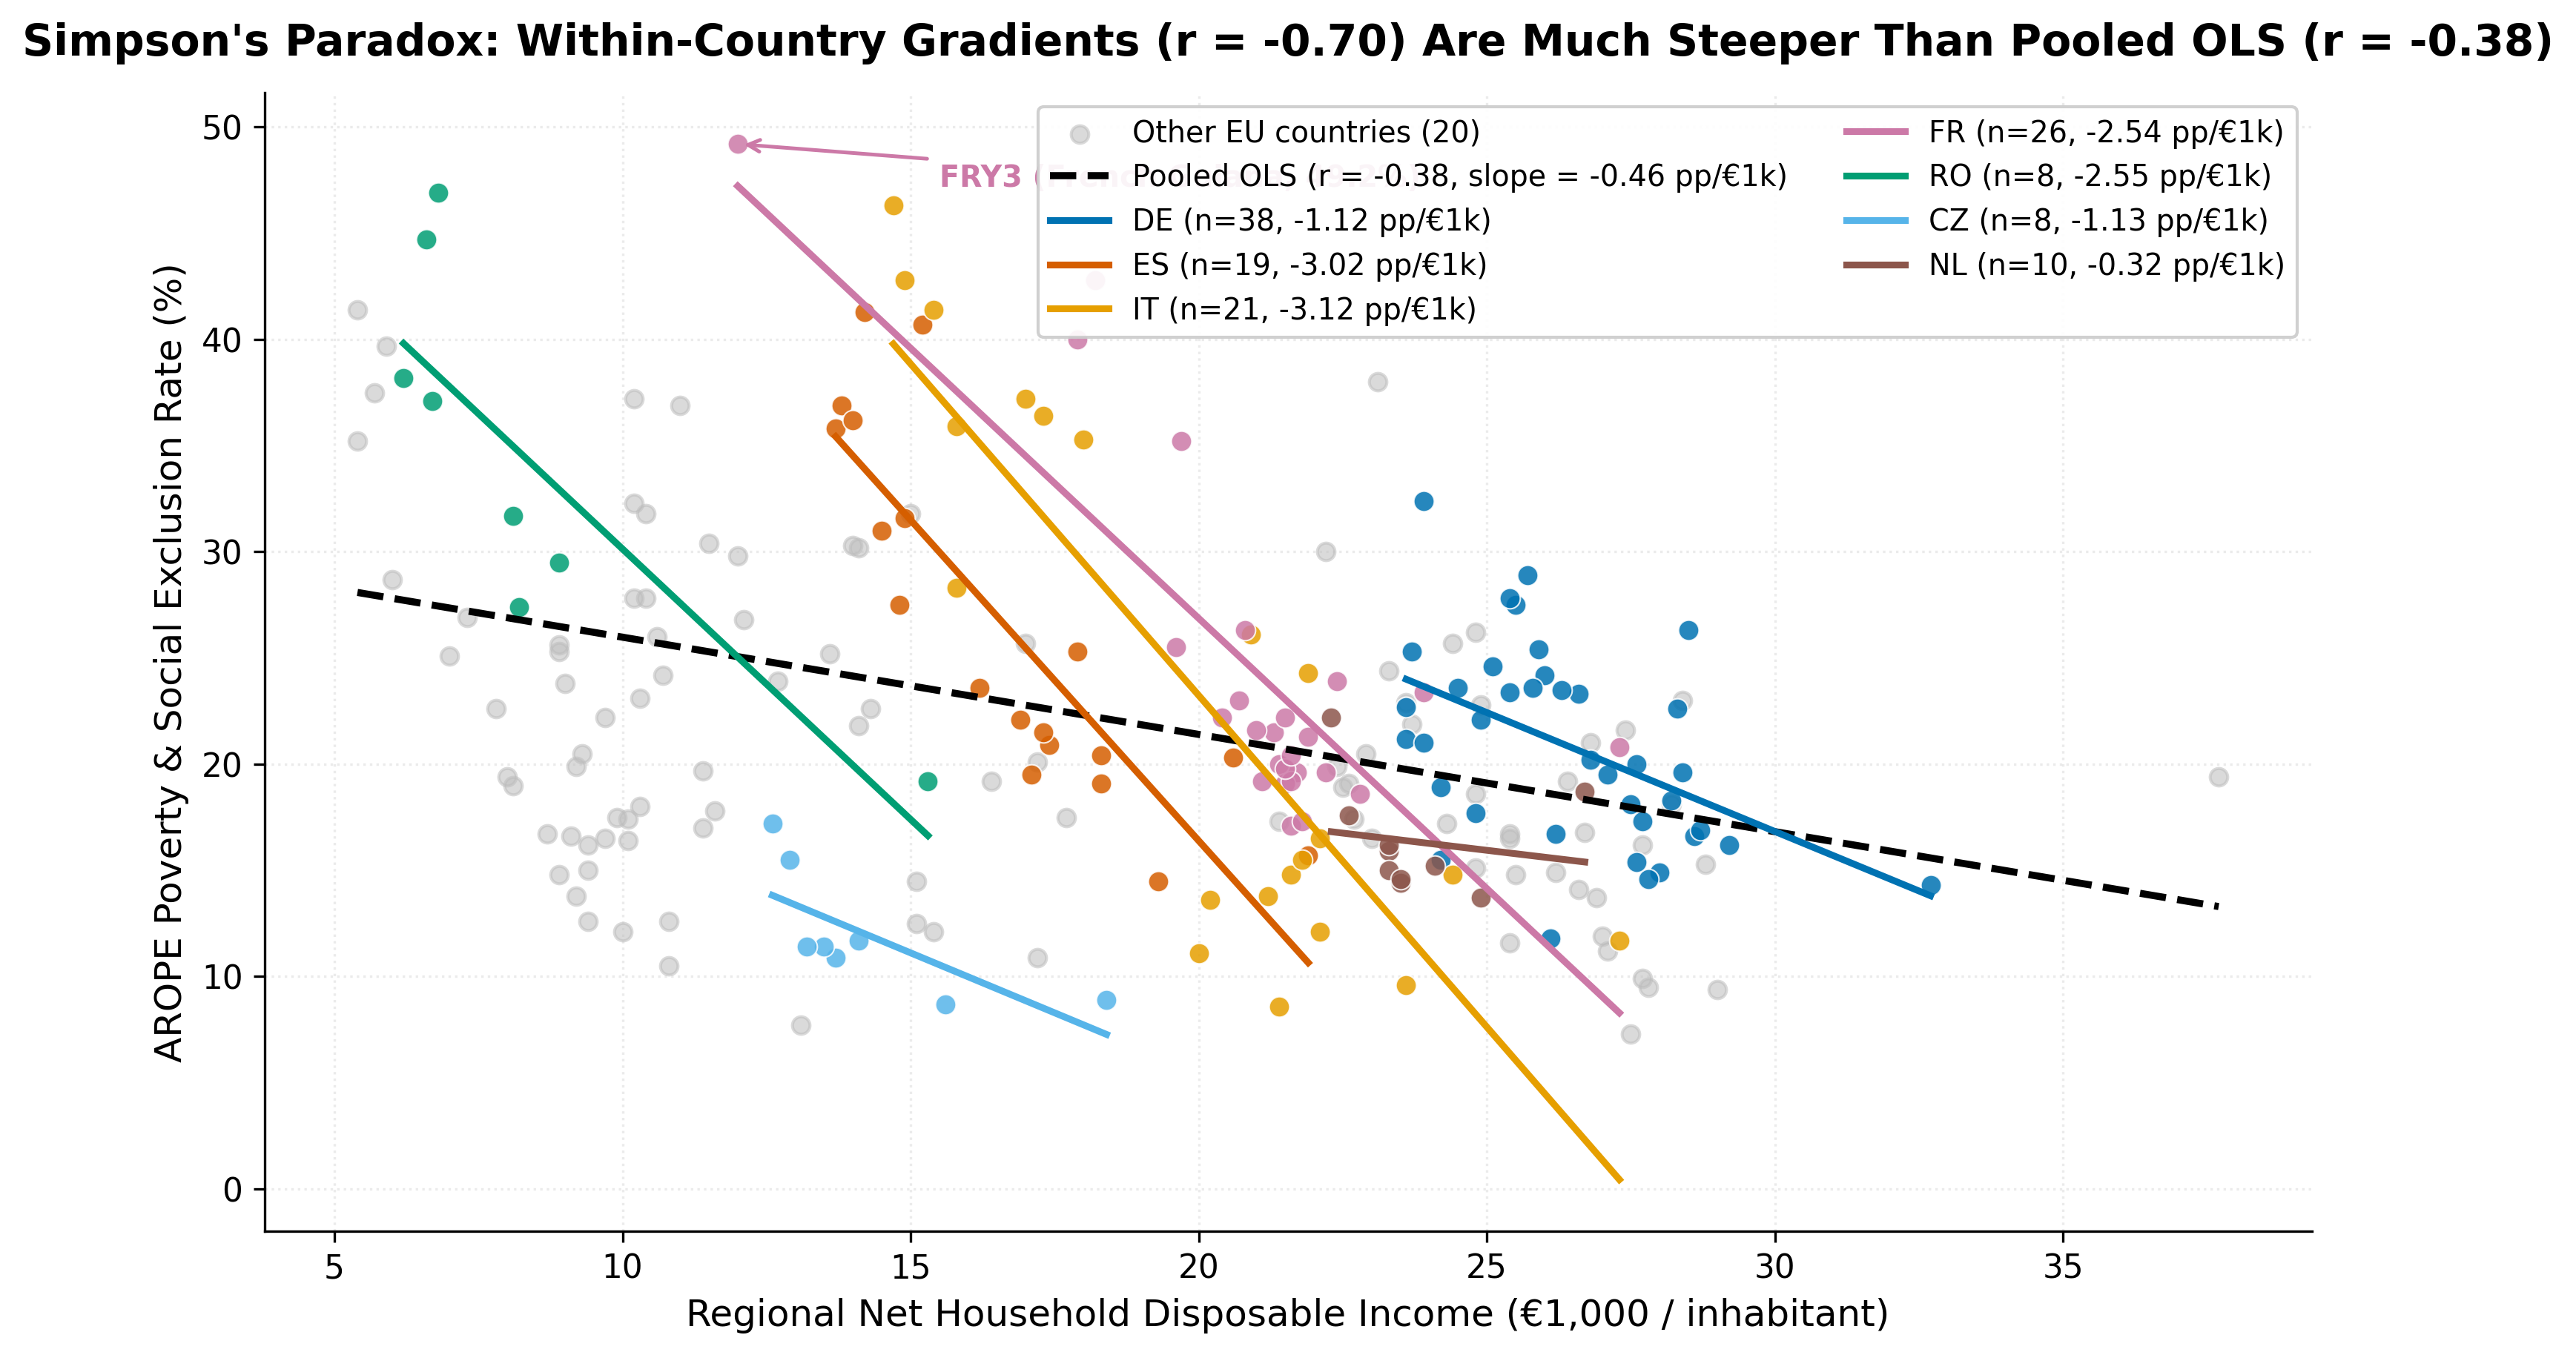
\includegraphics[width=0.88\textwidth]{01_eda_simpsons_paradox.png}
    \caption{Exploratory evidence of Simpson's paradox in 2022 Eurostat NUTS-2 data. Pooled OLS ($r = -0.38$) severely attenuates the stronger within-country income--poverty relationship ($r = -0.70$), which itself varies substantially across member states.}
    \label{fig:eda_simpson}
\end{figure}

\section{Model Formulation and Prior Specification}

Both models assume a continuous Gaussian likelihood for globally standardized AROPE $y_i$:
\begin{equation}
    y_i \sim \mathcal{N}(\mu_i, \sigma), \qquad i = 1, \dots, 232.
\end{equation}

\textbf{Model 1 (Complete Pooling Baseline)} ignores country boundaries and fits a single European intercept and slope:
\begin{equation}
    \mu_i = \alpha + \beta_{\text{inc}}\, x_{\text{inc}, i} + \beta_{\text{dens}}\, x_{\text{dens}, i}.
\end{equation}

\textbf{Model 2 (Hierarchical Varying Intercepts and Slopes)} introduces country-specific intercepts $\alpha_j = \mu_\alpha + u_{0j}$ and income slopes $\beta_{\text{inc}, j} = \mu_\beta + u_{1j}$ for $j = 1, \dots, 27$, while keeping urbanization $\beta_{\text{dens}}$ pooled across Europe:
\begin{align}
    \mu_i &= \alpha_{j[i]} + \beta_{\text{inc}, j[i]}\, x_{\text{inc}, i} + \beta_{\text{dens}}\, x_{\text{dens}, i}, \\
    \alpha_j &\sim \mathcal{N}(\mu_\alpha, \tau_\alpha), \qquad \beta_{\text{inc}, j} \sim \mathcal{N}(\mu_\beta, \tau_\beta).
\end{align}
\textbf{Implementation note on group-level structure:} Inspecting \texttt{print(model\_2)} in Bambi~0.13.0 \cite{capretto2022bambi} confirms that the formula syntax \texttt{(1 + disposable\_income\_scaled | country)} specifies \emph{independent} normal group-level effects ($\alpha_j \perp \beta_{\text{inc}, j}$ conditional on the hyperparameters), using a non-centered offset parameterization without an LKJ correlation matrix. We document this exact structure here so the mathematical specification matches the sampled posterior 1-to-1.

Table~\ref{tab:priors} lists every prior across both models. Zero improper flat priors or undocumented library defaults are used. We calibrate the income slope prior to $\mathcal{N}(0, 1.5)$---wider than a tight $\mathcal{N}(0, 0.5)$---because the EDA revealed steep within-country standardized slopes reaching $-2.5$ to $-3.4$ under Simpson's paradox. Prior predictive simulations on the original AROPE (\%) scale (Appendix Figure~\ref{fig:app_prior}) confirm that both models generate plausible European poverty rates (95\% prior predictive intervals $[-23.0\%, 68.7\%]$ for Model~1 and $[-28.3\%, 72.6\%]$ for Model~2, medians $22.2\%$ and $21.2\%$) without artificial hard bounds.

\begin{table}[H]
\centering
\caption{Explicit proper weakly informative priors for Model~1 and Model~2 on globally $z$-standardized variables.}
\label{tab:priors}
\begin{tabular}{llll}
\toprule
Parameter & Role & Model~1 & Model~2 \\
\midrule
$\alpha$ / $\mu_\alpha$ & Global intercept & $\mathcal{N}(0, 1.5)$ & $\mathcal{N}(0, 1.5)$ \\
$\beta_{\text{inc}}$ / $\mu_\beta$ & Global income slope & $\mathcal{N}(0, 1.5)$ & $\mathcal{N}(0, 1.5)$ \\
$\beta_{\text{dens}}$ & Log density slope & $\mathcal{N}(0, 1.0)$ & $\mathcal{N}(0, 1.0)$ \\
$\tau_\alpha$ & Country intercept SD & --- & $\text{HalfNormal}(1.0)$ \\
$\tau_\beta$ & Country income slope SD & --- & $\text{HalfNormal}(1.0)$ \\
$\sigma$ & Residual SD & $\text{Exponential}(1.0)$ & $\text{Exponential}(1.0)$ \\
\bottomrule
\end{tabular}
\end{table}

Listing~\ref{lst:bambi} shows the core Bambi/PyMC specification and sampling call used for Model~2.

\begin{lstlisting}[style=pybda,caption={Bambi specification and NUTS sampling configuration for Model~2 (PyMC 5.12 / Bambi 0.13).},label={lst:bambi}]
FORMULA_M2 = (
    "arope_scaled ~ disposable_income_scaled + log_pop_density_scaled "
    "+ (1 + disposable_income_scaled | country)"
)
BASE_PRIORS_M2 = {
    "Intercept": bmb.Prior("Normal", mu=0, sigma=1.5),
    "disposable_income_scaled": bmb.Prior("Normal", mu=0, sigma=1.5),
    "log_pop_density_scaled": bmb.Prior("Normal", mu=0, sigma=1.0),
    "1|country": bmb.Prior("Normal", mu=0, sigma=bmb.Prior("HalfNormal", sigma=1.0)),
    "disposable_income_scaled|country": bmb.Prior(
        "Normal", mu=0, sigma=bmb.Prior("HalfNormal", sigma=1.0)
    ),
    "sigma": bmb.Prior("Exponential", lam=1.0),
}
model_2 = bmb.Model(FORMULA_M2, data=df, family="gaussian", priors=BASE_PRIORS_M2)
idata_2 = model_2.fit(
    draws=2000, tune=1000, chains=4, target_accept=0.95,
    random_seed=42, omit_offsets=False, idata_kwargs={"log_likelihood": True}
)
\end{lstlisting}

\section{MCMC Inference and Convergence Diagnostics}

All models---primary fits, the conditional Student-$t$ check, and all five prior sensitivity refits---were sampled using PyMC's No-U-Turn Sampler (NUTS) with identical settings: 4 independent chains, 1,000 warmup iterations, and 2,000 post-warmup draws per chain (8,000 total draws), with \texttt{random\_seed=42}. We set \texttt{target\_accept=0.95} to prevent step-size divergences in the hierarchical variance funnel induced by single-region countries, and \texttt{omit\_offsets=False} so posterior predictive draws condition faithfully on the fitted non-centered country offsets rather than re-sampling them from the prior.

Table~\ref{tab:convergence} summarizes worst-case convergence diagnostics across all parameters of every fitted model following Vehtari et al. \cite{vehtari2021rank}. Every run satisfies $\max\hat{R} \le 1.004$ (threshold $\le 1.01$), minimum Bulk-ESS $\ge 1{,}852$ and Tail-ESS $\ge 3{,}026$ (threshold $> 400$), zero divergent transitions, and minimum E-BFMI $\ge 0.55$ (threshold $\ge 0.30$). Figure~\ref{fig:conv} confirms visually that the 4-chain rank histograms are uniform across all population parameters and variance components in both models, indicating thorough mixing and reliable Monte Carlo estimation.

\begin{table}[H]
\centering
\caption{Worst-case MCMC convergence diagnostics across all primary, robustness, and prior sensitivity fits (4 chains $\times$ 2,000 post-warmup draws each).}
\label{tab:convergence}
\begin{tabular}{lcccccc}
\toprule
Model / Refit & Params & Max $\hat{R}$ & Min Bulk-ESS & Min Tail-ESS & Divergences & Min E-BFMI \\
\midrule
Model 1 (Pooled, Base) & 4 & 1.001 & 8,406 & 5,484 & 0 & 1.00 \\
Model 2 (Hierarchical, Base) & 114 & 1.002 & 2,030 & 3,026 & 0 & 0.64 \\
Model 2-$t$ (Student-$t$ Check) & 115 & 1.004 & 1,936 & 3,151 & 0 & 0.67 \\
\midrule
M1 Skeptical: $\beta_{\text{inc}} \sim \mathcal{N}(0, 0.1)$ & 4 & 1.001 & 8,697 & 5,554 & 0 & 1.02 \\
M1 Wider: $\beta_{\text{inc}} \sim \mathcal{N}(0, 3.0)$ & 4 & 1.001 & 8,794 & 5,354 & 0 & 1.01 \\
M2 Skeptical Slope: $\mu_\beta \sim \mathcal{N}(0, 0.1)$ & 114 & 1.003 & 1,852 & 3,860 & 0 & 0.55 \\
M2 Tight Hyper: $\tau \sim \text{HN}(0.3)$ & 114 & 1.002 & 2,669 & 4,374 & 0 & 0.74 \\
M2 Wide Hyper: $\tau \sim \text{HN}(2.0)$ & 114 & 1.002 & 2,187 & 3,127 & 0 & 0.64 \\
\bottomrule
\end{tabular}
\end{table}

\begin{figure}[H]
    \centering
    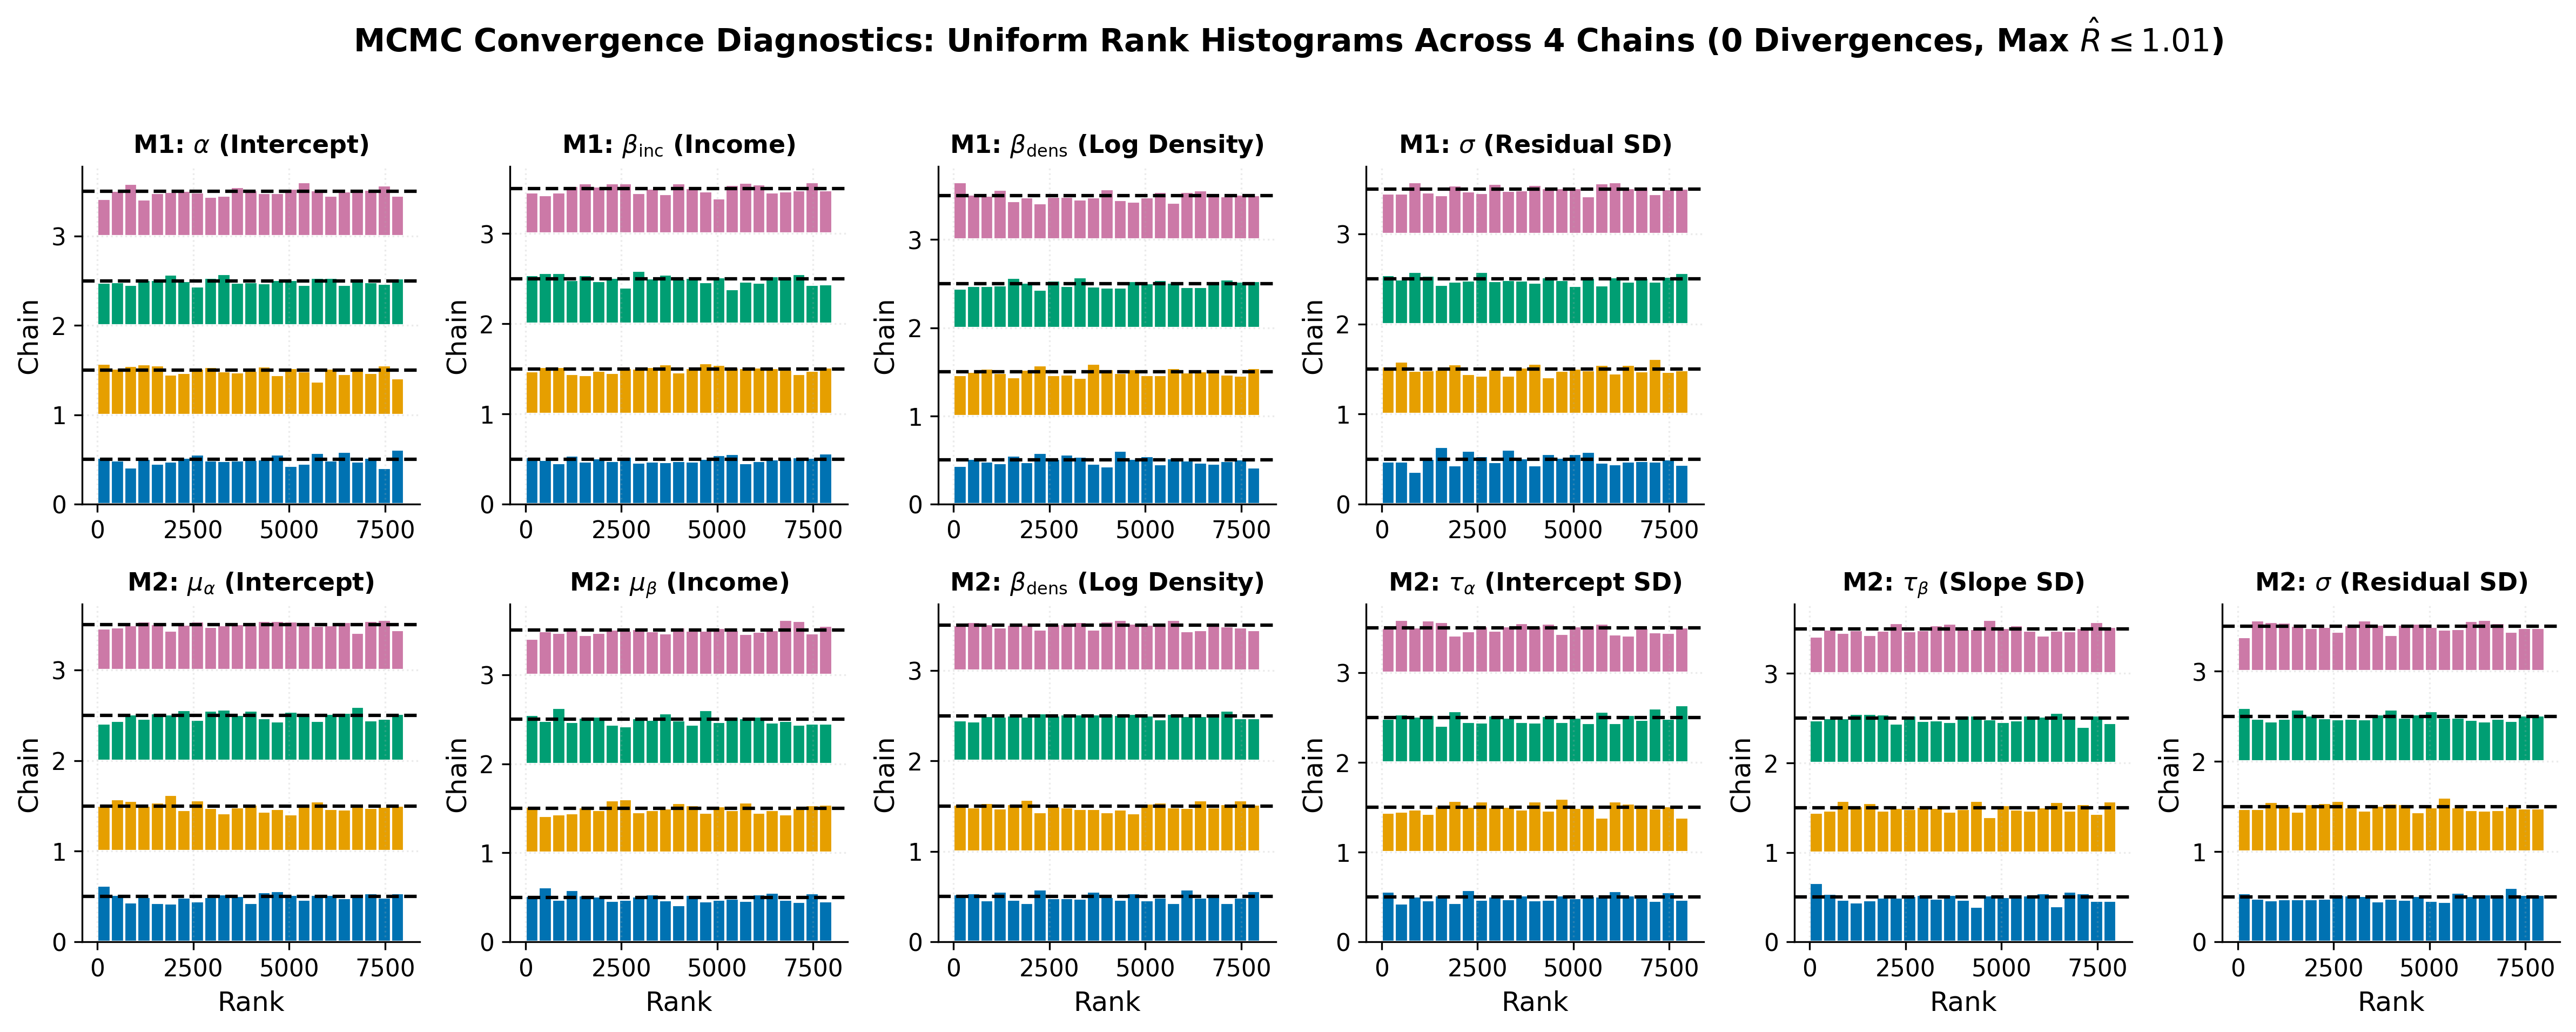
\includegraphics[width=0.95\textwidth]{04_convergence_diagnostics.png}
    \caption{Vehtari-style rank histograms across 4 MCMC chains for all Model~1 parameters (top) and Model~2 population and variance parameters (bottom). Uniformity across chains confirms clean mixing.}
    \label{fig:conv}
\end{figure}

\section{Model Validation: Posterior Predictive Checks and Prior Sensitivity}

\subsection{Posterior Predictive Checks (All Models)}

We assess generative adequacy on the original AROPE (\%) scale using marginal KDE overlays, LOO-PIT ECDF calibration, tail test statistics, and country-grouped checks \cite{gabry2019visualization}. In Figure~\ref{fig:ppc_kde}, Model~2 reproduces both the location and right-shouldered shape of the empirical AROPE distribution far more closely than Model~1, and its LOO-PIT ECDF curve remains well inside the 94\% uniform calibration envelope, whereas Model~1 shifts the modal peak and dips to the lower calibration boundary.

Tail test statistics (Appendix Figure~\ref{fig:app_ppc_stats}) show that Model~2 captures the extreme upper-tail observation \texttt{FRY3} ($49.2\%$) cleanly, with a replicated maximum median of $46.9\%$ ($p_B = 0.24$, vs.\ $45.3\%$, $p_B = 0.15$ for Model~1). Both models underestimate overall empirical right-skewness ($0.93$), though Model~2 moves substantially closer (median replicated skewness $0.37$ vs.\ $0.01$ for Model~1, $p_B = 0.00$)---an expected limitation of a symmetric Gaussian likelihood on a bounded rate.

\begin{figure}[H]
    \centering
    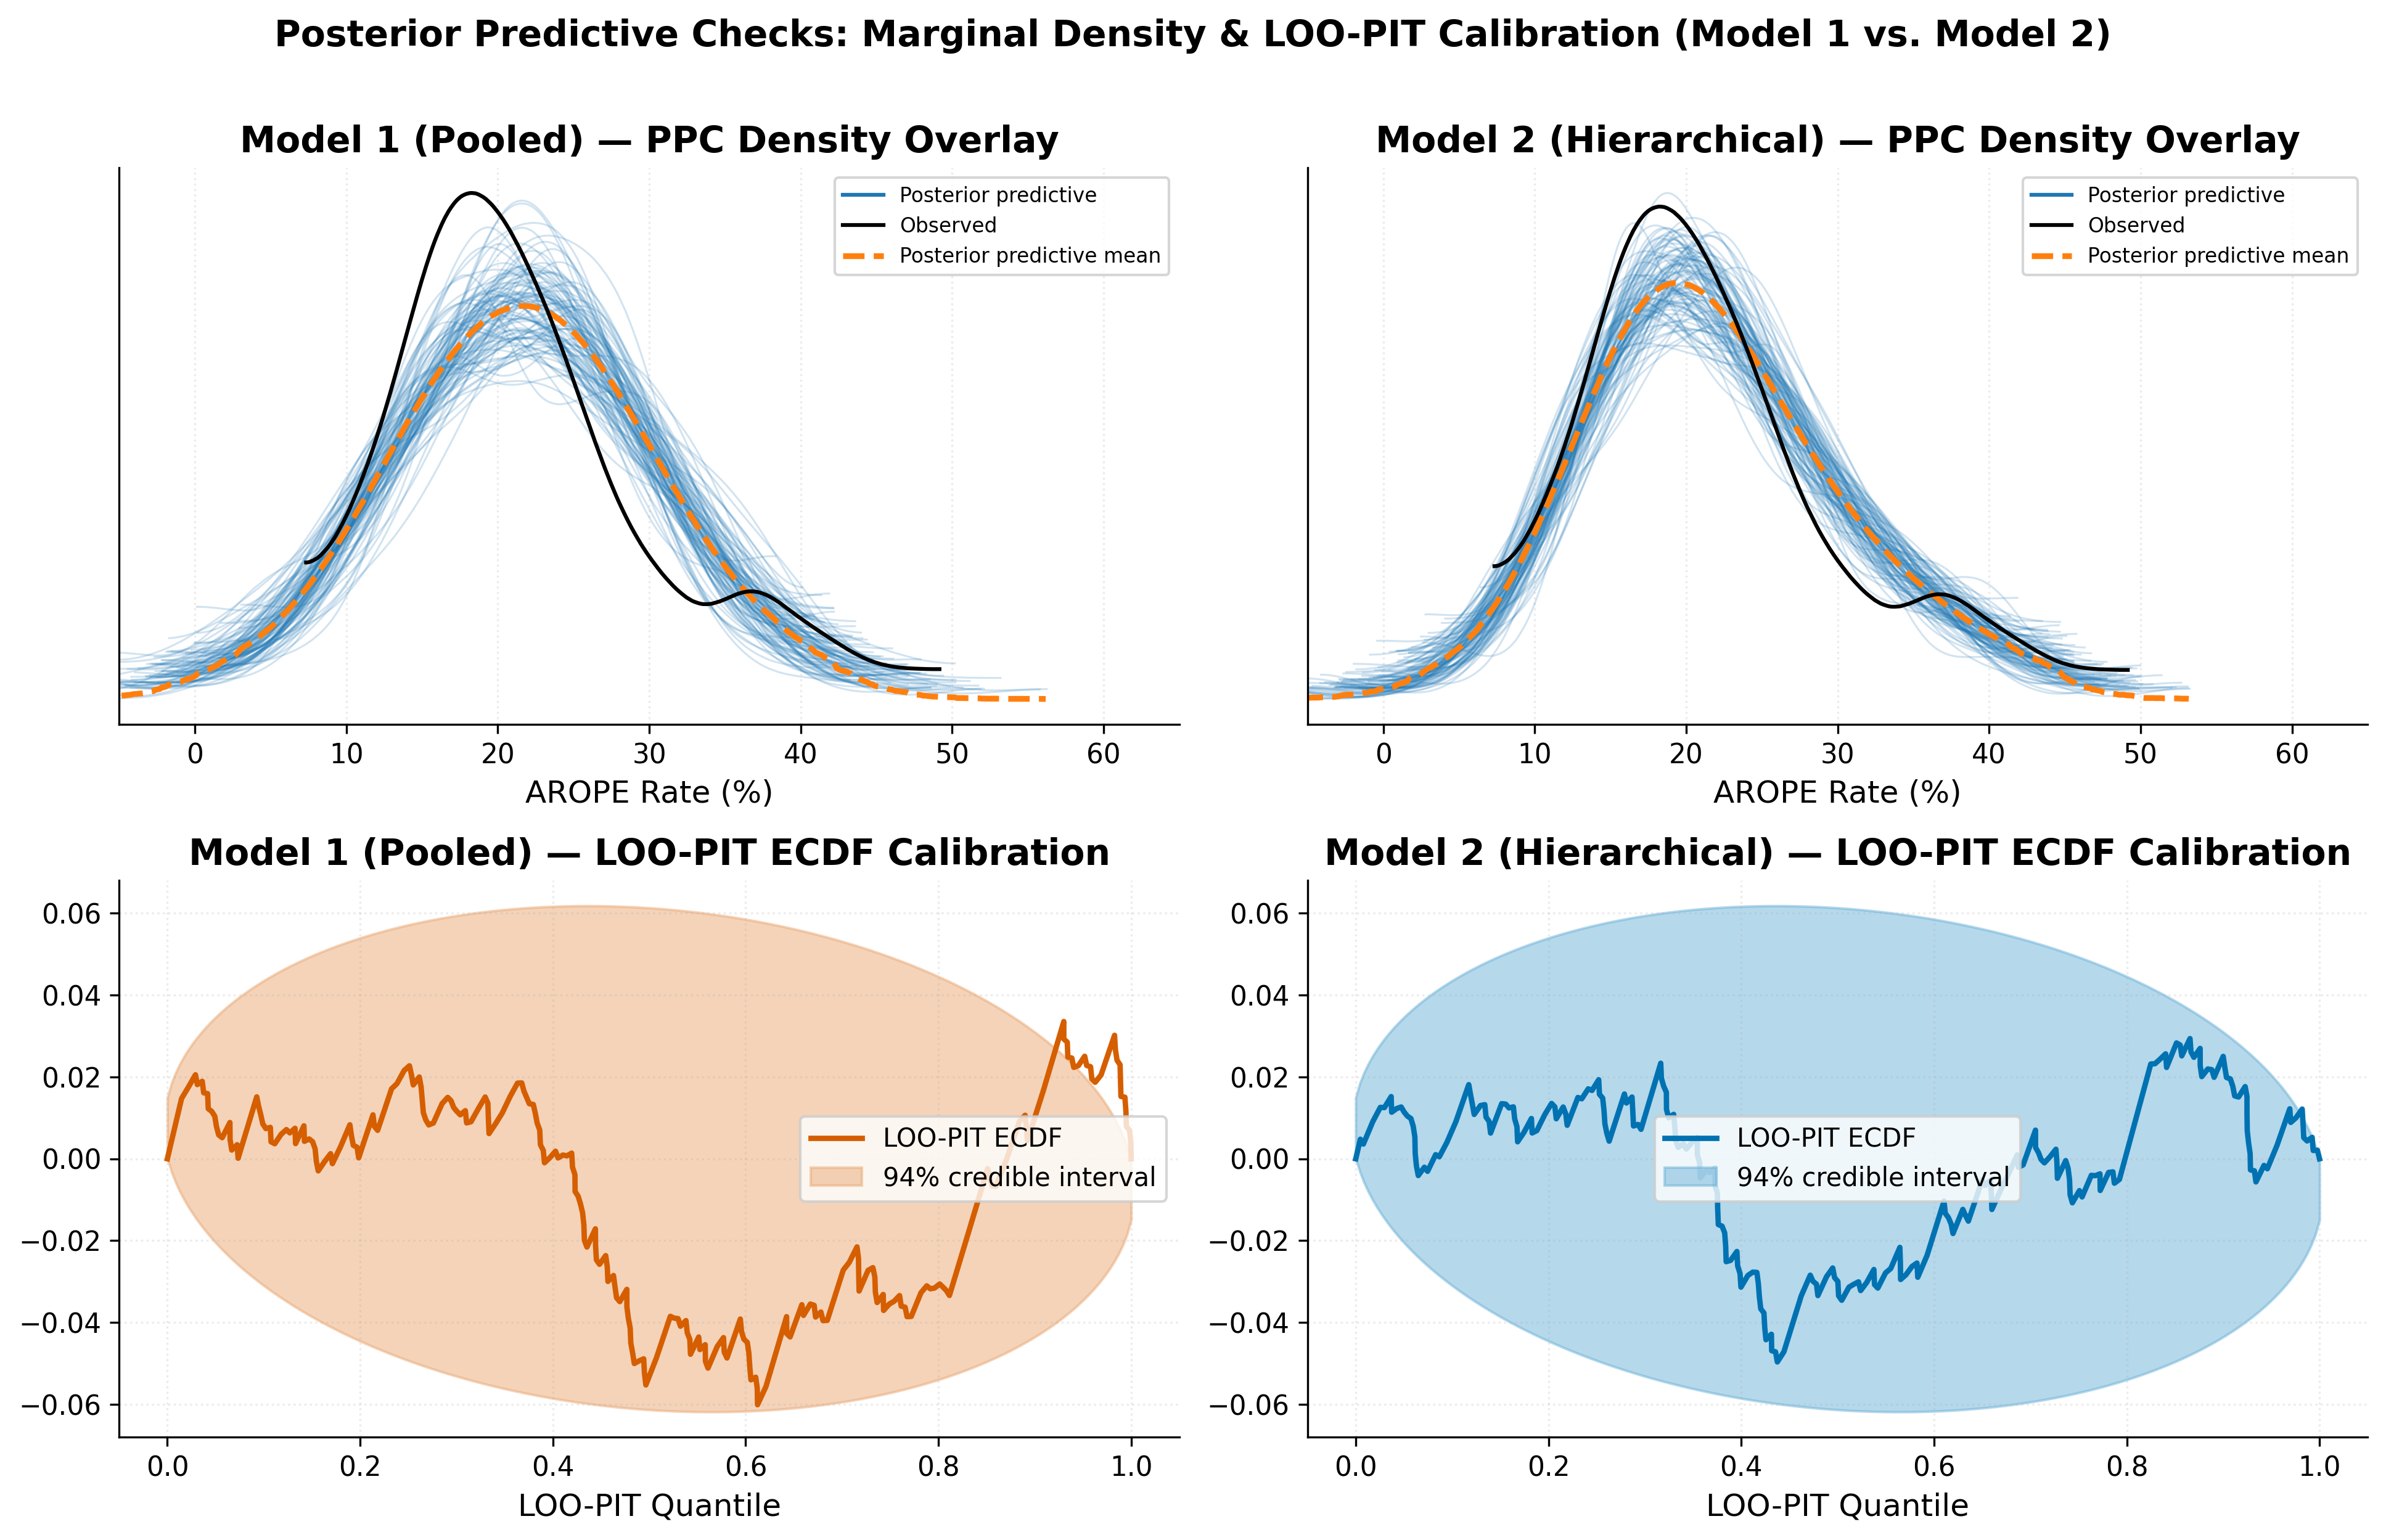
\includegraphics[width=0.90\textwidth]{05_ppc_kde_and_loopit.png}
    \caption{Marginal posterior predictive KDE overlays (top, AROPE \%) and LOO-PIT ECDF calibration plots (bottom) comparing Model~1 and Model~2.}
    \label{fig:ppc_kde}
\end{figure}

The grouped country-level check (Figure~\ref{fig:ppc_country}) provides the clearest structural diagnostic. Model~1 fails to cover 6 of 27 observed country means within its 95\% predictive intervals (coverage $21/27 = 77.8\%$), systematically underpredicting high-poverty countries (\texttt{RO}, \texttt{BG}) and overpredicting low-poverty Central European states (\texttt{CZ}, \texttt{SI}, \texttt{SK}, \texttt{PL}). Model~2 achieves $27/27$ ($100.0\%$) coverage with noticeably sharper predictive intervals.

\begin{figure}[H]
    \centering
    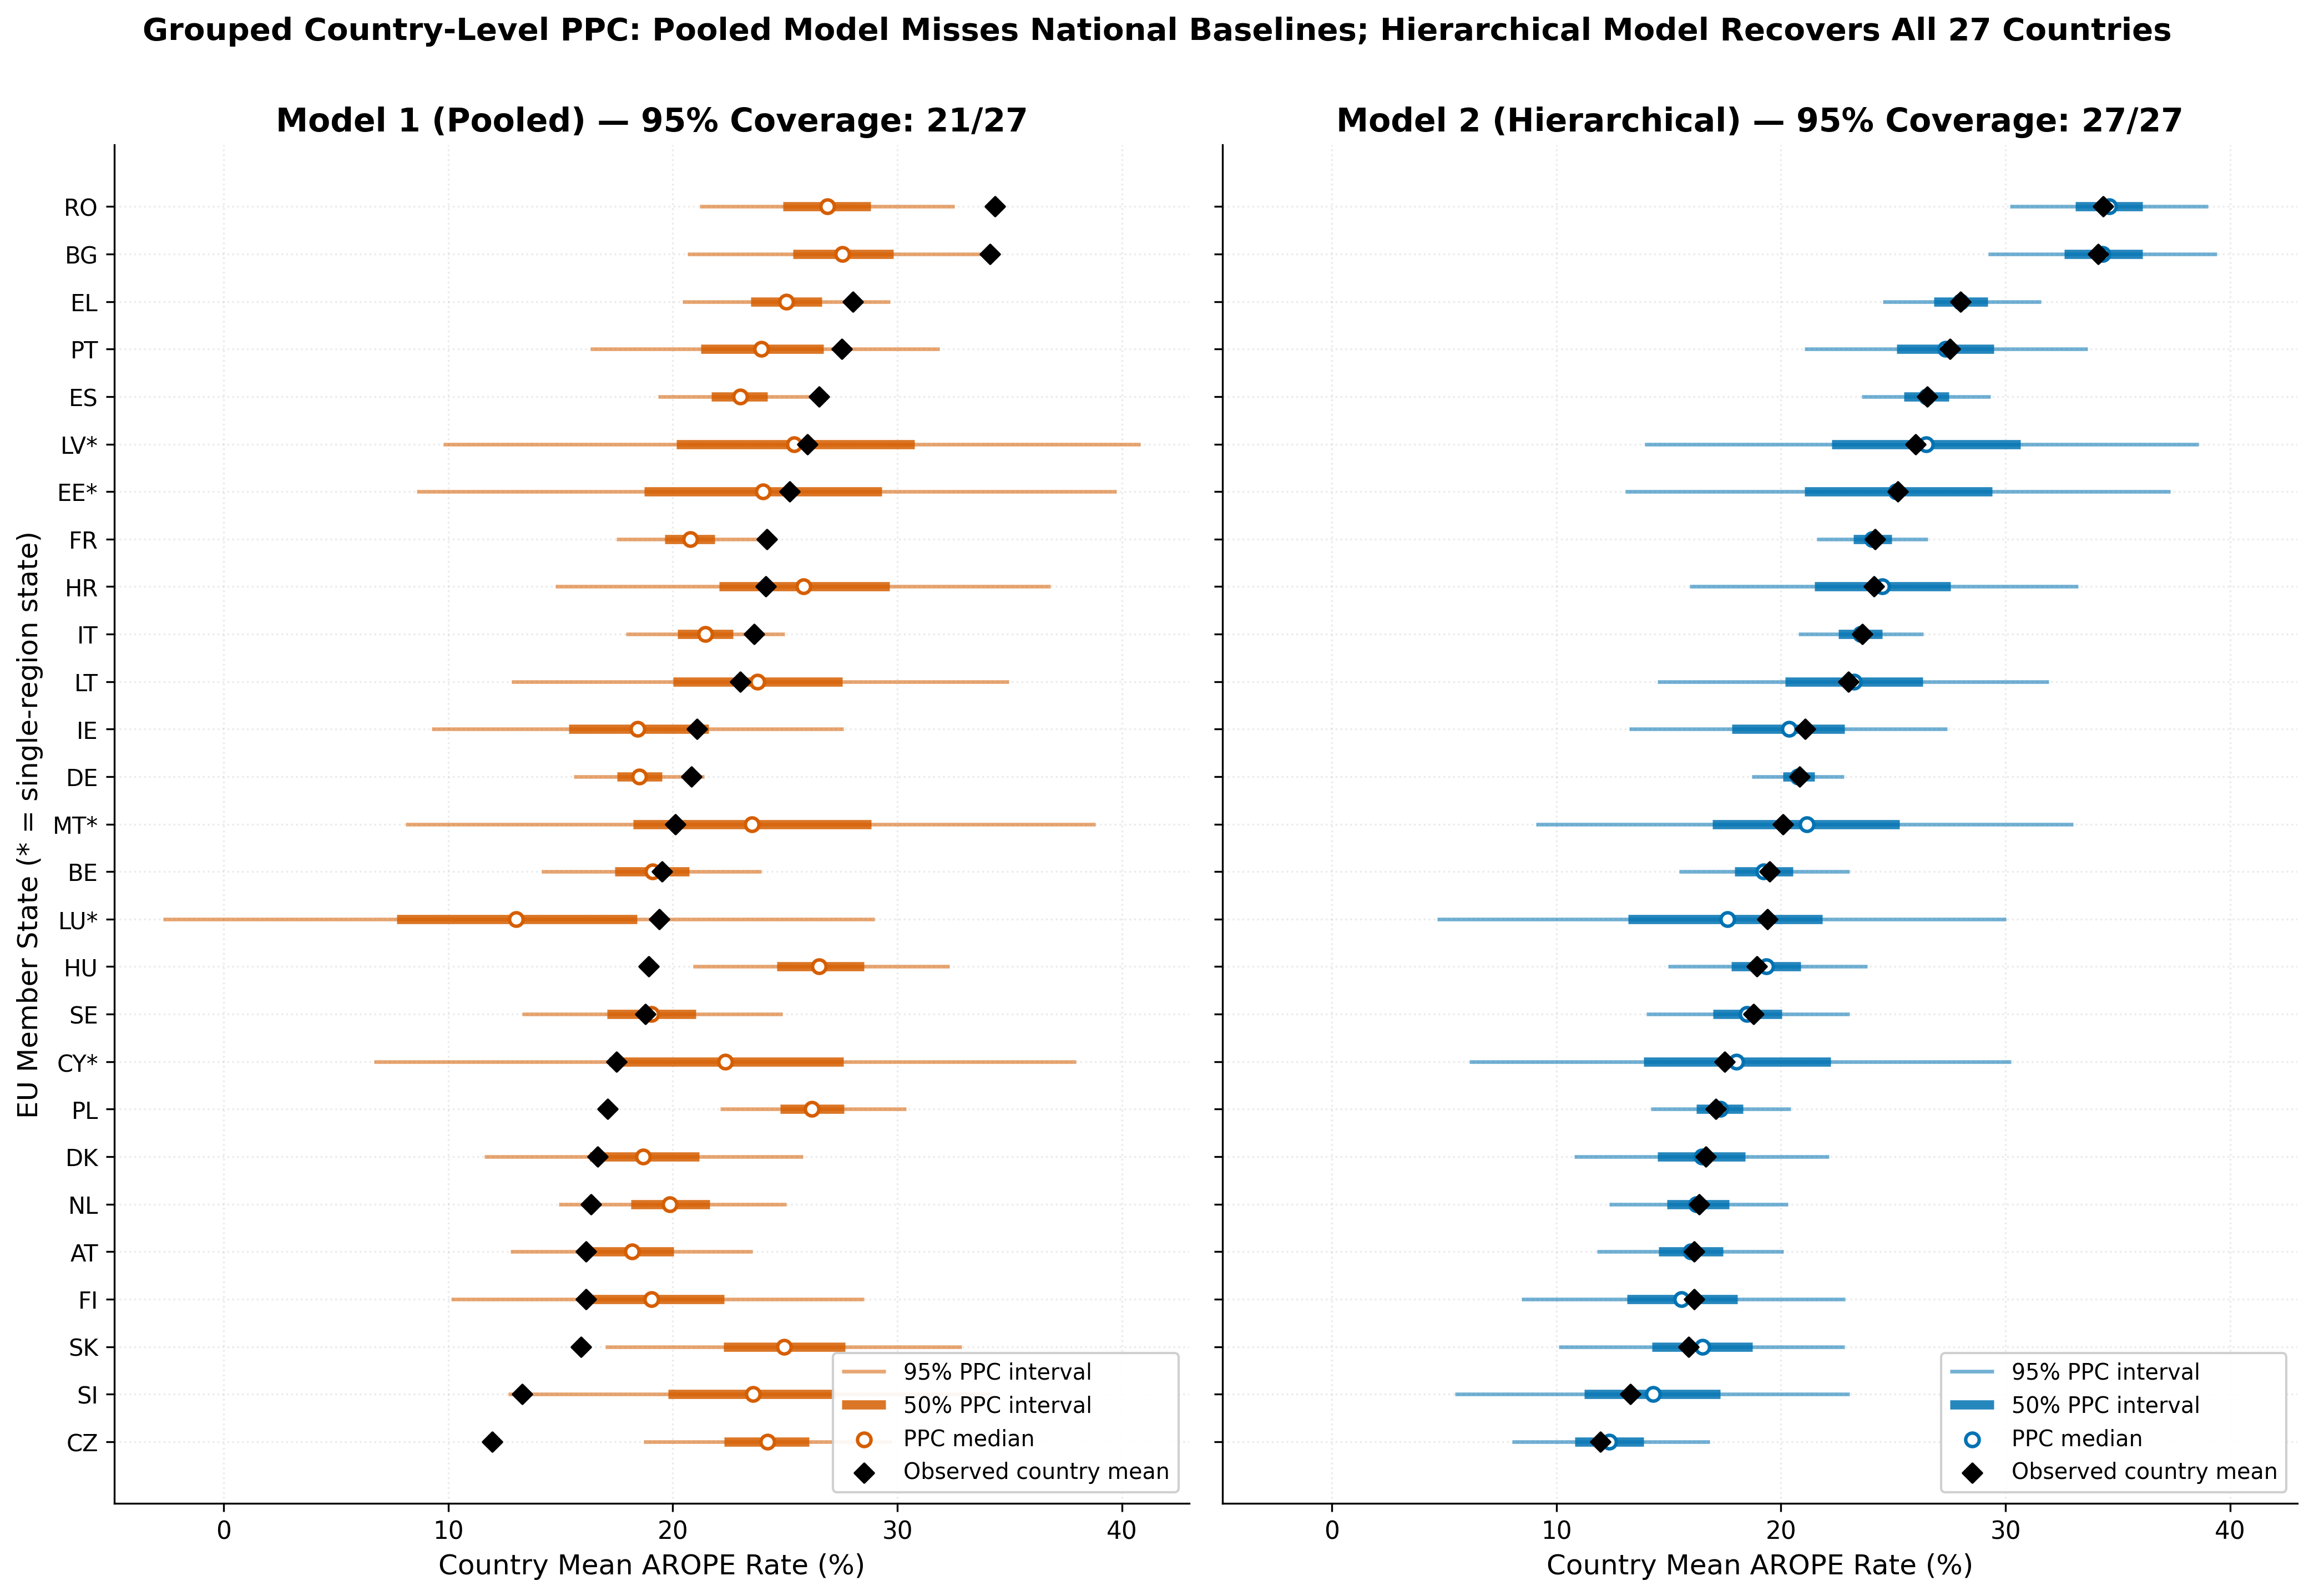
\includegraphics[width=0.92\textwidth]{07_ppc_grouped_by_country.png}
    \caption{Grouped country-level posterior predictive checks across all 27 EU member states (* denotes single-region states). Model~1 misses 6 national baselines (77.8\% coverage); Model~2 recovers all 27 (100.0\%).}
    \label{fig:ppc_country}
\end{figure}

\subsection{Prior Sensitivity Analysis (All Models)}

To verify that inferences are data-driven, we re-fit both models under alternative prior regimes (Figure~\ref{fig:sens}). For Model~1, widening $\beta_{\text{inc}}$ to $\mathcal{N}(0, 3.0)$ leaves the posterior identical ($-0.39$, 95\% HDI $[-0.51, -0.26]$ vs.\ base $[-0.52, -0.27]$), and even a strongly skeptical $\mathcal{N}(0, 0.1)$ prior preserves a clearly negative slope ($-0.27$, $[-0.38, -0.17]$).

For Model~2, varying the group-level hyperpriors across nearly an order of magnitude---$\text{HalfNormal}(0.3)$, $\text{HalfNormal}(1.0)$, and $\text{HalfNormal}(2.0)$---yields highly stable posteriors for $\mu_\beta$ ($-1.19$, $-1.35$, $-1.36$) and $\beta_{\text{dens}}$ ($0.20$, $0.22$, $0.22$), with $\tau_\alpha$ and $\tau_\beta$ shifting only modestly under $\text{HalfNormal}(0.3)$. Under the deliberately extreme skeptical prior $\mu_\beta \sim \mathcal{N}(0, 0.1)$, the tight zero-centered prior pulls the population mean toward $-0.14$ (95\% HDI $[-0.33, 0.05]$) because only $J = 27$ countries inform $\mu_\beta$; simultaneously, $\tau_\beta$ expands from $0.67$ to $1.18$ ($[0.79, 1.61]$) so that individual country deviations $u_{1j}$ absorb the strongly negative empirical slopes. This textbook prior--data conflict diagnostic confirms both why $\mathcal{N}(0, 0.1)$ is miscalibrated and why our weakly informative $\mathcal{N}(0, 1.5)$ baseline is appropriate.

\begin{figure}[H]
    \centering
    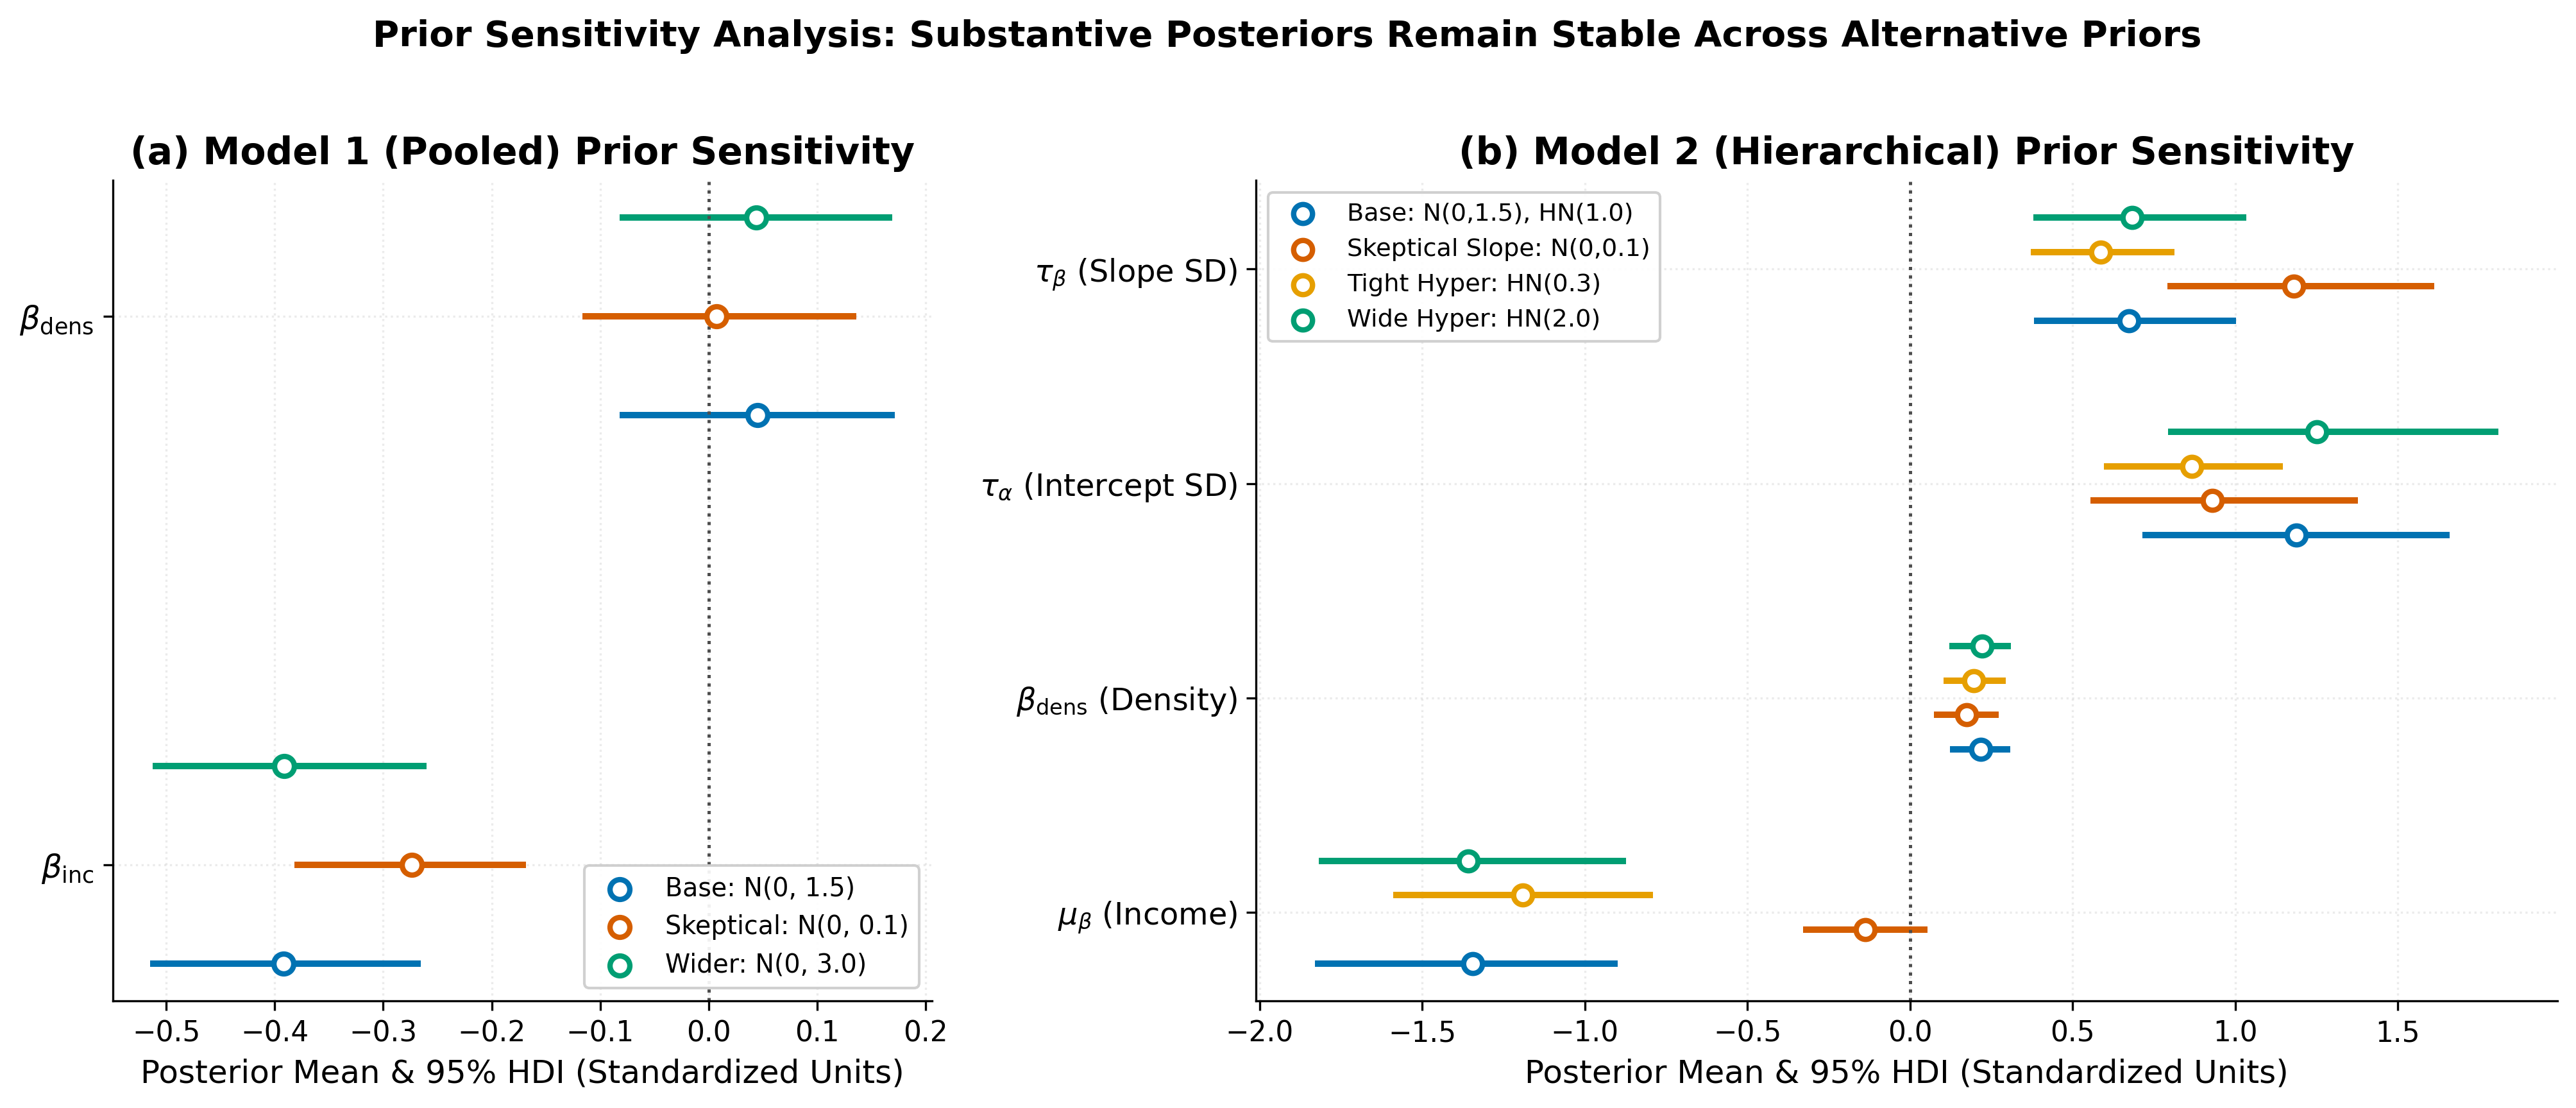
\includegraphics[width=0.90\textwidth]{08_prior_sensitivity.png}
    \caption{Prior sensitivity comparison (posterior mean and 95\% HDI in standardized units) for Model~1 (left) and Model~2 (right). Reasonable hyperprior changes leave all substantive conclusions intact.}
    \label{fig:sens}
\end{figure}

\section{Model Comparison and Tail Robustness}

We evaluate out-of-sample predictive accuracy via Pareto-Smoothed Importance Sampling Leave-One-Out Cross-Validation (PSIS-LOO-CV) \cite{vehtari2017practical}, complemented by practical prediction errors in real AROPE percentage points and Bayesian $R^2$. Table~\ref{tab:comparison} summarizes all comparison metrics.

\begin{table}[H]
\centering
\caption{PSIS-LOO-CV comparison and practical predictive performance (in real AROPE percentage points) for Model~1, Model~2, and the conditional Student-$t$ robustness check.}
\label{tab:comparison}
\begin{tabular}{lcccccccc}
\toprule
Model & $\text{ELPD}_{\text{LOO}}$ & $p_{\text{LOO}}$ & $\Delta\text{ELPD} \pm \text{SE}$ & Weight & $\hat{k} > 0.7$ & RMSE (pp) & MAE (pp) & Bayes $R^2$ \\
\midrule
Model 2 (Hier.) & $-208.4$ & 35.5 & $0.0 \pm 0.0$ & 0.99 & 4 / 232 & 4.18 & 3.34 & $0.71 \pm 0.02$ \\
Model 2-$t$ (Check) & $-210.2$ & 38.5 & $-1.8 \pm 1.2$ & 0.00 & 5 / 232 & --- & --- & --- \\
Model 1 (Pooled) & $-315.2$ & 4.9 & $-106.9 \pm 13.0$ & 0.01 & 0 / 232 & 7.79 & 6.00 & $0.15 \pm 0.04$ \\
\bottomrule
\end{tabular}
\end{table}

Model~2 decisively outperforms Model~1 by $\Delta\text{ELPD}_{\text{LOO}} = +106.9 \pm 13.0$ ($> 8\text{ SE}$, stacking weight $0.99$). Practically, accounting for country hierarchies nearly halves posterior mean prediction error (RMSE drops from $7.79$ to $4.18\text{ pp}$; MAE from $6.00$ to $3.34\text{ pp}$) and lifts Bayesian $R^2$ from $0.15 \pm 0.04$ to $0.71 \pm 0.02$.

Figure~\ref{fig:khat} inspects pointwise Pareto $\hat{k}$ reliability. While Model~1 has zero $\hat{k} > 0.7$ observations ($\max \hat{k} = 0.35$), Model~2 flags 4 observations above $0.7$: \texttt{LU00} ($\hat{k} = 1.09$), \texttt{MT00} ($0.94$), \texttt{EE00} ($0.84$), and \texttt{LV00} ($0.72$). Crucially, \emph{all four are single-region countries ($n_j = 1$)}, where leaving out the sole region removes 100\% of the data informing that country's random effects and forces out-of-group prediction. To verify that high $\hat{k}$ does not stem from heavy-tailed residual misspecification (e.g., \texttt{FRY3}), we fitted a conditional hierarchical Student-$t$ model (Model~2-$t$, $\nu \sim \text{Gamma}(2, 0.1)$). The posterior for degrees of freedom concentrates at $\nu = 27.0 \pm 14.7$ (95\% HDI $[5.5, 55.5]$), indicating near-Gaussian tails; Model~2-$t$ yields no ELPD gain ($\Delta\text{ELPD} = -1.8 \pm 1.2$) and retains 5 observations with $\hat{k} > 0.7$. Because the 4 high-$\hat{k}$ points reflect structural $n_j = 1$ leverage and the ELPD advantage over Model~1 exceeds $8\text{ SE}$, we retain the parsimonious Gaussian Model~2 as our preferred specification.

\begin{figure}[H]
    \centering
    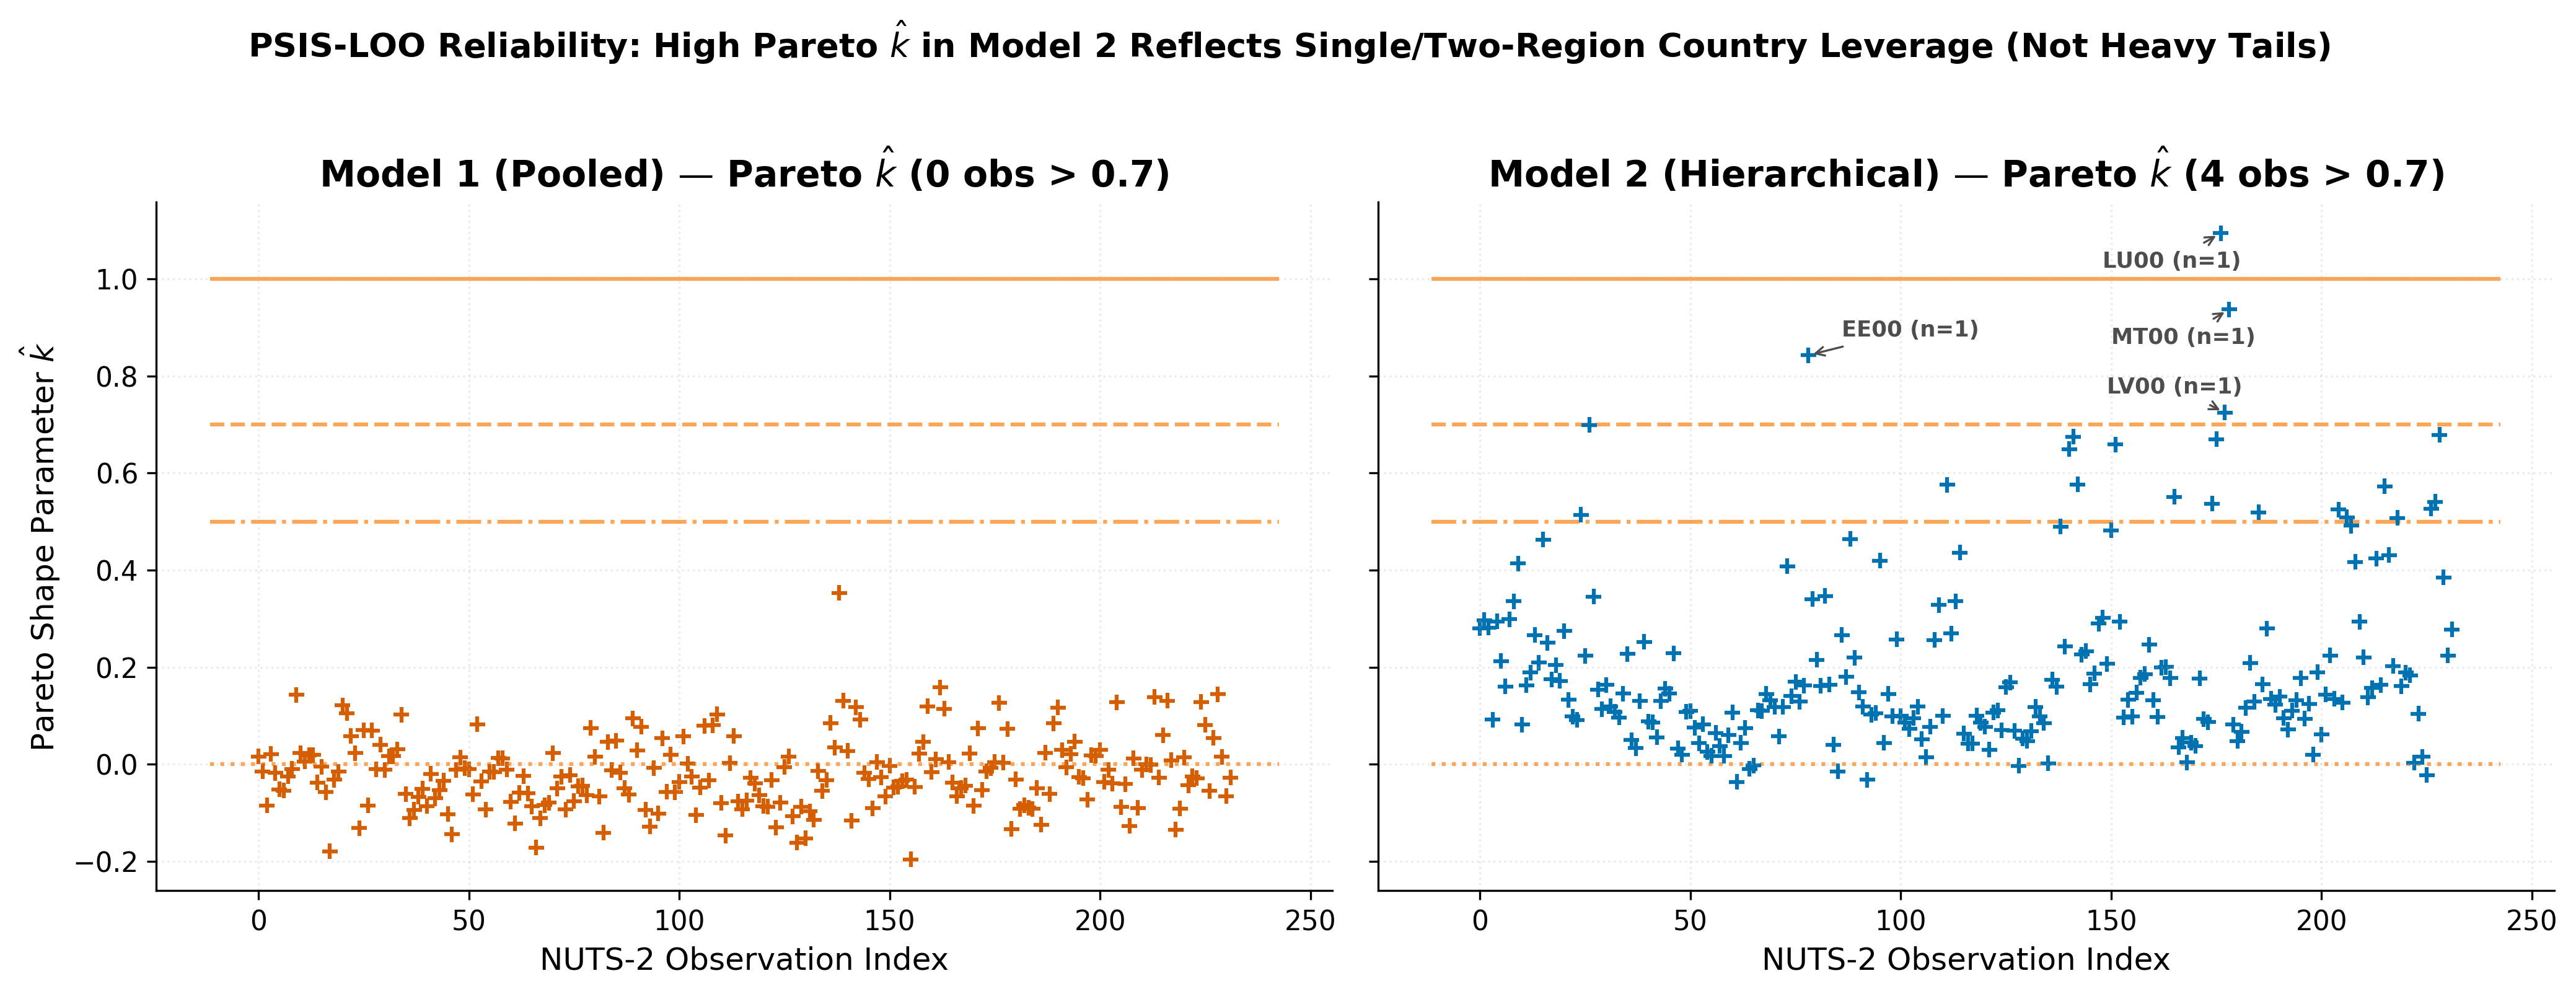
\includegraphics[width=0.90\textwidth]{09_loo_pareto_k.png}
    \caption{Pointwise Pareto $\hat{k}$ diagnostics for PSIS-LOO-CV. All four $\hat{k} > 0.7$ observations in Model~2 are single-region states ($n_j = 1$), reflecting structural out-of-group leverage rather than heavy-tailed outliers.}
    \label{fig:khat}
\end{figure}

\section{Substantive Results and Policy Interpretation}

Table~\ref{tab:posterior} reports Model~2's population-level posteriors in both standardized units and back-transformed policy units (where $\Delta\text{AROPE}_{\text{pp per \euro{}1k}} = \beta_{\text{inc}, j} \times (\text{SD}_{\text{AROPE}} / \text{SD}_{\text{inc}}) \times 1000$). Across Europe, a +\euro{}1,000 increase in regional net disposable income is associated with an average $-1.63\text{ pp}$ reduction in AROPE (95\% HDI $[-2.22, -1.09]$). Cross-country variation is substantial in both baseline poverty ($\tau_\alpha = 10.02\text{ pp}$) and income sensitivity ($\tau_\beta = 0.82\text{ pp}$ per \euro{}1,000), exceeding within-country residual variation ($\sigma = 4.57\text{ pp}$).

\begin{table}[H]
\centering
\caption{Model~2 population-level posterior summary in standardized and back-transformed real units (mean, SD, and 95\% HDI).}
\label{tab:posterior}
\begin{tabular}{lccccl}
\toprule
Parameter & Std.\ Mean (SD) & Std.\ 95\% HDI & Real Mean (SD) & Real 95\% HDI & Real Unit \\
\midrule
Global intercept ($\mu_\alpha$) & $-0.37\;(0.25)$ & $[-0.86, 0.14]$ & $18.78\;(2.15)$ & $[14.58, 23.02]$ & AROPE \% at avg.\ cov. \\
Global income ($\mu_\beta$) & $-1.35\;(0.24)$ & $[-1.83, -0.90]$ & $-1.63\;(0.29)$ & $[-2.22, -1.09]$ & pp per +\euro{}1,000 \\
Urbanization ($\beta_{\text{dens}}$) & $+0.22\;(0.05)$ & $[0.12, 0.31]$ & $+1.10\;(0.24)$ & $[0.62, 1.55]$ & pp per $2\times$ density \\
Intercept SD ($\tau_\alpha$) & $1.19\;(0.24)$ & $[0.71, 1.66]$ & $10.02\;(2.05)$ & $[6.03, 13.99]$ & pp across countries \\
Slope SD ($\tau_\beta$) & $0.67\;(0.16)$ & $[0.38, 1.00]$ & $0.82\;(0.20)$ & $[0.46, 1.22]$ & pp/\euro{}1k across countries \\
Residual SD ($\sigma$) & $0.54\;(0.03)$ & $[0.49, 0.60]$ & $4.57\;(0.24)$ & $[4.10, 5.04]$ & pp within countries \\
\bottomrule
\end{tabular}
\end{table}

Figure~\ref{fig:caterpillar} displays the country-specific income slopes across all 27 member states. Regional income is most strongly protective in Southern, Eastern, and federal-regionalized states with stark internal disparities: Italy ($-2.95\text{ pp}$/\euro{}1k, 95\% HDI $[-3.46, -2.34]$), Spain ($-2.65$, $[-3.43, -1.86]$), France ($-2.64$, $[-3.30, -2.00]$), Romania ($-2.34$, $[-3.23, -1.44]$), and Belgium ($-2.26$, $[-3.22, -1.37]$). Conversely, slopes are less than half as steep in well-informed corporatist and Nordic welfare states such as Germany ($-1.15$, $[-1.79, -0.44]$), Denmark ($-1.21$, $[-2.51, 0.26]$), and the Netherlands ($-1.36$). Single-region states (\texttt{CY}, \texttt{EE}, \texttt{LV}, \texttt{MT}, \texttt{LU}) exhibit wide credible intervals and strong partial-pooling shrinkage toward $\mu_\beta$ (visualized against noisy unpooled OLS in Appendix Figure~\ref{fig:app_shrinkage}).

\begin{figure}[H]
    \centering
    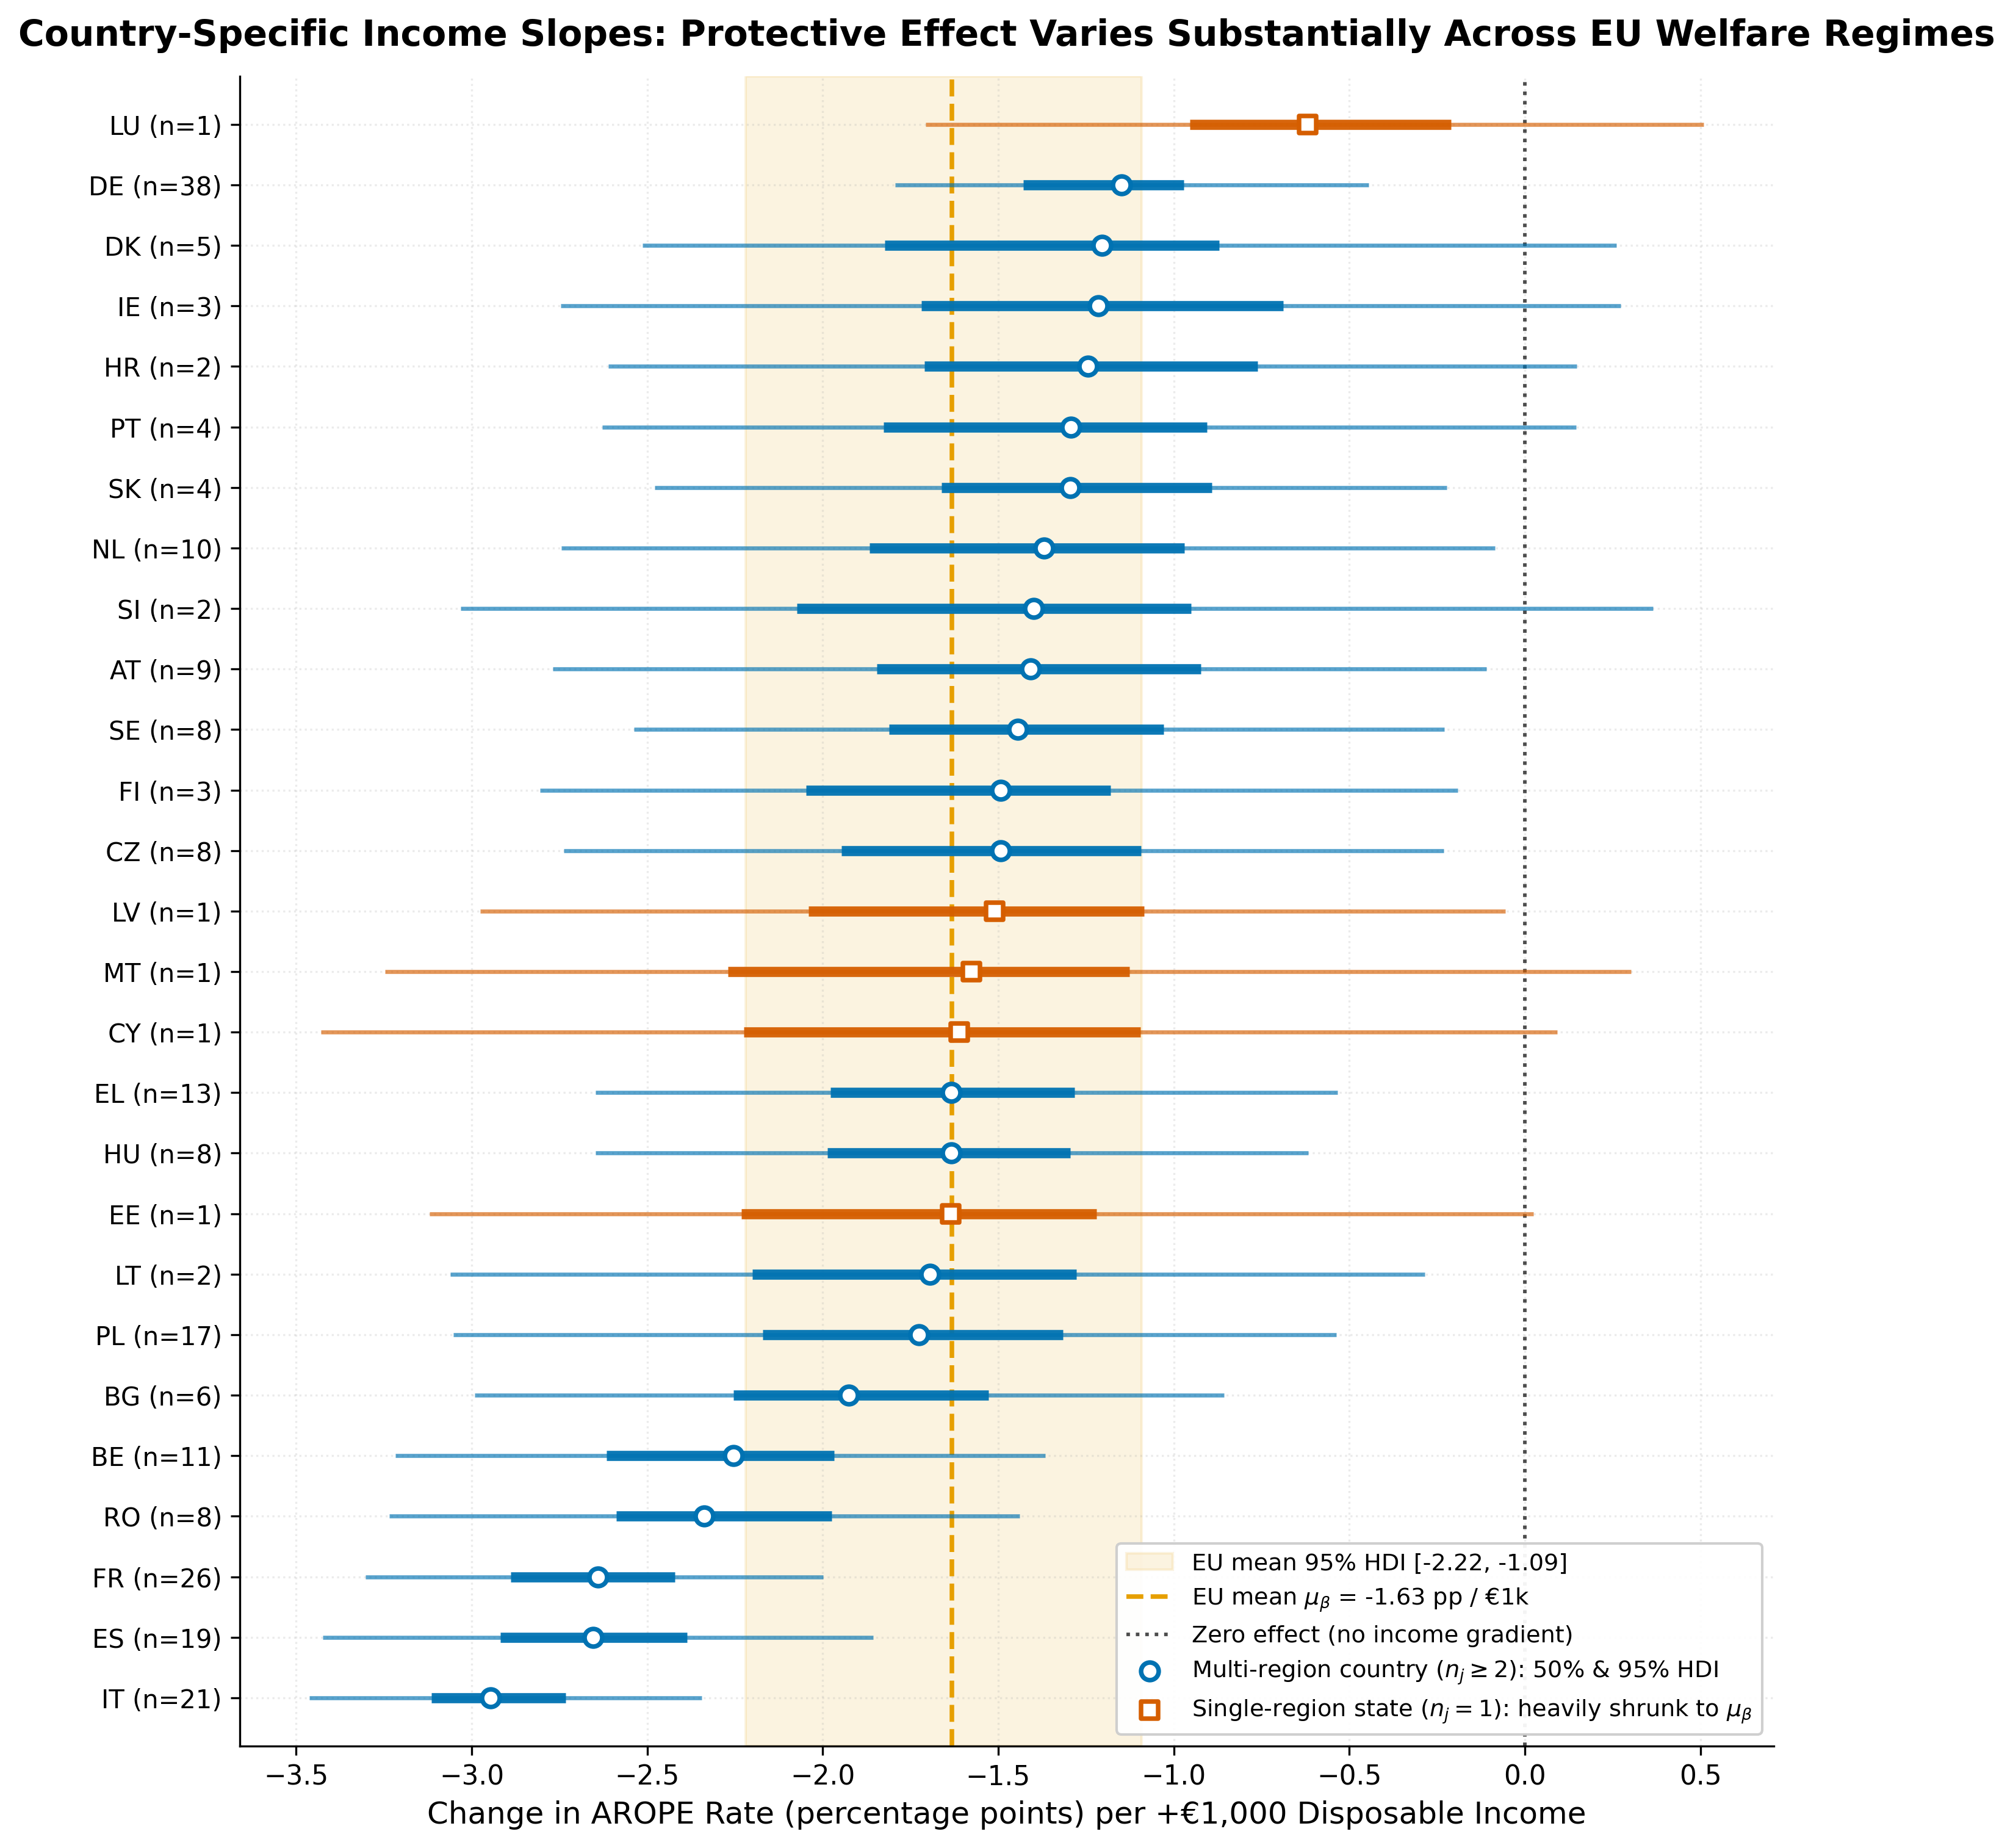
\includegraphics[width=0.88\textwidth]{10_country_slopes_caterpillar.png}
    \caption{Country-specific income slopes ($\beta_{\text{inc}, j}$ in pp AROPE per +\euro{}1,000) sorted by posterior mean, with 50\% (thick) and 95\% (thin) HDIs. Single-region states ($n_j = 1$) are highlighted in vermilion.}
    \label{fig:caterpillar}
\end{figure}

Controlling for regional disposable income and country hierarchies uncovers a clear \textbf{urbanization paradox}: doubling regional population density is associated with a $+1.10\text{ pp}$ \emph{increase} in AROPE (95\% HDI $[0.62, 1.55]$). Although metropolitan hubs have higher nominal wages, once income is held constant, dense urban areas exhibit higher housing-cost pressures, sharper intraurban inequality, and concentrated pockets of social exclusion.

Finally, Figure~\ref{fig:counterfactual} propagates full parameter uncertainty into a concrete policy scenario: an increase of +\euro{}5,000 in regional disposable income across five contrasting welfare regimes. Expected AROPE reductions are nearly twice as large in Spain ($-13.3\text{ pp}$, 95\% HDI $[-17.1, -9.3]$) and Romania ($-11.7\text{ pp}$, $[-16.2, -7.2]$, both $P(\Delta < -5\text{ pp}) = 1.00$) as in Germany ($-5.7\text{ pp}$, $[-9.0, -2.2]$), the Netherlands ($-6.8\text{ pp}$, $[-13.7, -0.4]$), and Finland ($-7.5\text{ pp}$, $[-14.0, -1.0]$).

\begin{figure}[H]
    \centering
    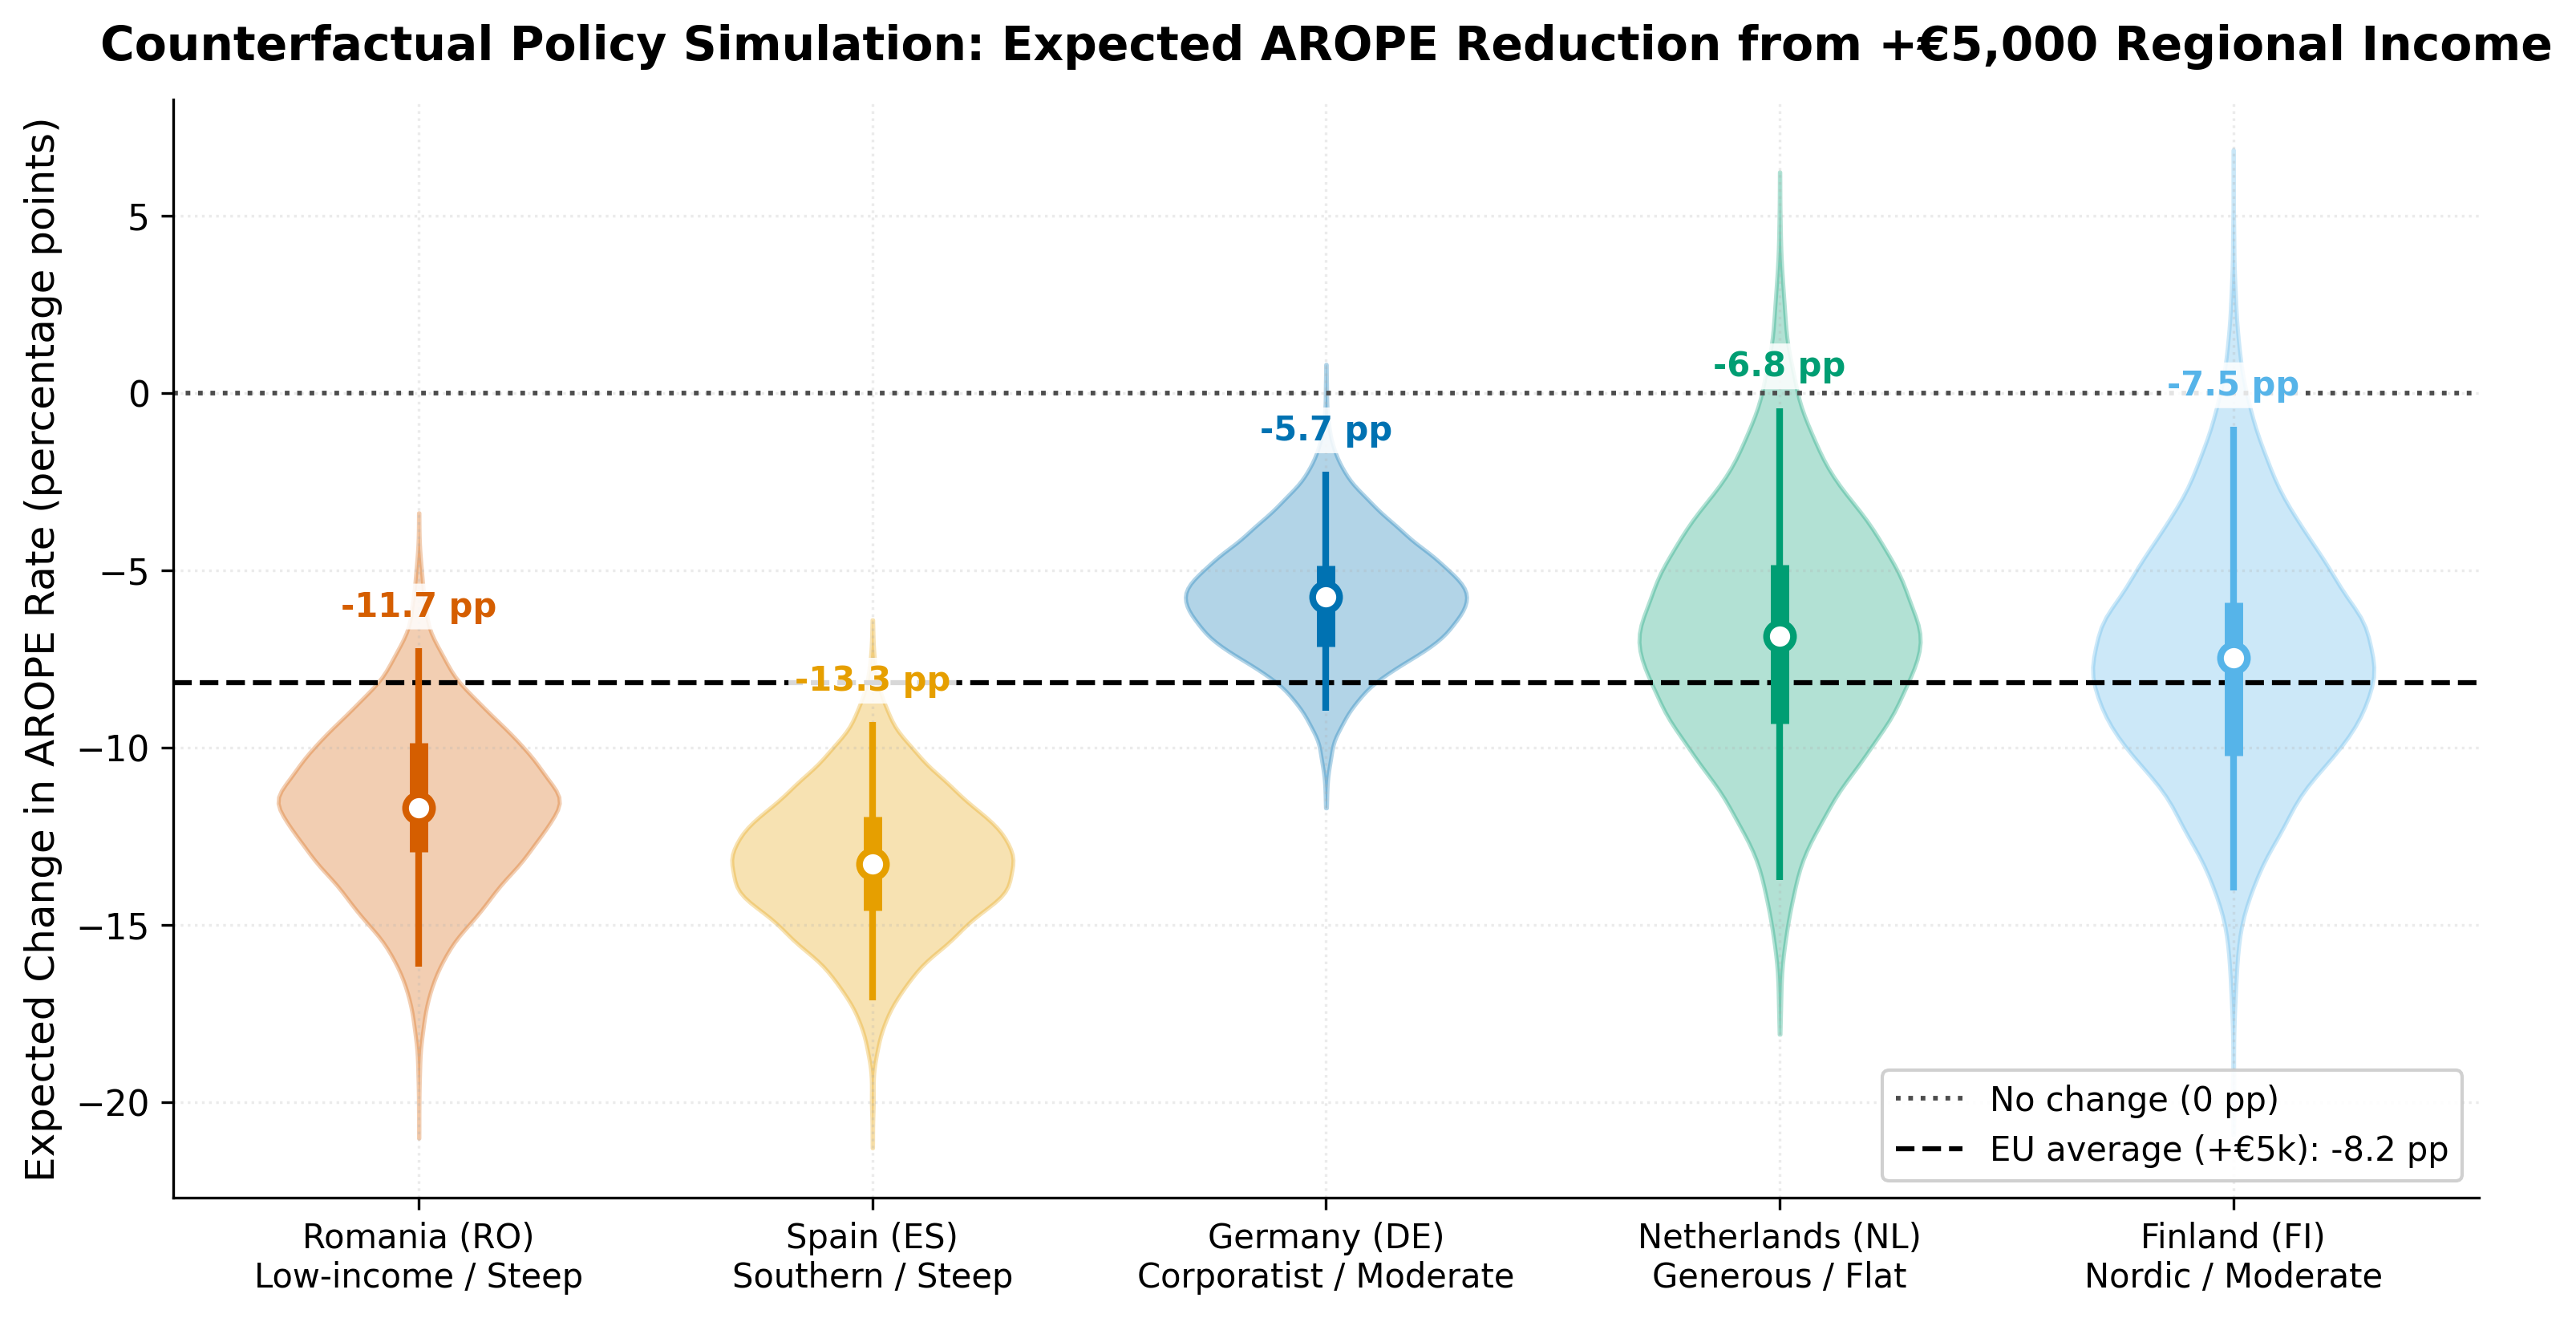
\includegraphics[width=0.88\textwidth]{12_counterfactual_scenarios.png}
    \caption{Counterfactual posterior simulation of expected AROPE change (pp) from a +\euro{}5,000 regional disposable income increase across five contrasting EU welfare regimes (violin densities with 50\% and 95\% HDIs).}
    \label{fig:counterfactual}
\end{figure}

\section{Discussion, Limitations, and Reflection}

\textbf{Main Takeaways.} Returning to our research question, higher regional disposable income \emph{does not} protect against poverty and social exclusion equally across Europe. While income is protective across virtually every EU country ($\mu_\beta = -1.63\text{ pp}$/\euro{}1k), national welfare regimes strongly moderate both baseline deprivation ($\tau_\alpha = 10.02\text{ pp}$) and regional income gradients ($\tau_\beta = 0.82\text{ pp}$/\euro{}1k), with gradients in Southern and Eastern Europe more than twice as steep as in Germany, Denmark, or the Netherlands. Ignoring national hierarchies induces severe Simpson's paradox, misses 22\% of national baselines, and forfeits over $100$ ELPD points and $56$ percentage points of Bayesian $R^2$.

\textbf{Limitations and Future Work.} Four limitations qualify these findings: (1) our 2022 cross-sectional design identifies conditional associations rather than causal income interventions; (2) NUTS-2 aggregation is subject to the ecological fallacy, masking household-level deprivation inside affluent cities; (3) because AROPE's income component uses 60\% of \emph{national} median income, national baselines partly reflect relative rather than absolute deprivation; and (4) Bambi's independent group-level parameterization omits intercept--slope correlation, while the symmetric Gaussian likelihood mildly underestimates global right-skewness. Natural extensions include implementing a correlated LKJ(2) prior in pure PyMC, adding spatial CAR/BYM2 random effects for cross-border NUTS-2 adjacency, and modeling multi-year Eurostat panels on a logit/Beta scale.

\textbf{Group Reflection.} Building the analysis iteratively---from initial EDA through prior calibration, rank-plot diagnostics, PPCs, and the conditional Student-$t$ check---demonstrated how diagnostic failures actively guide modeling decisions. In particular, auditing Bambi's default parameterization, resolving the \texttt{omit\_offsets=False} subtlety for accurate PPCs, and diagnosing the four single-region $\hat{k} > 0.7$ observations deepened our practical understanding of hierarchical Bayesian workflow.

\textbf{AI Usage Disclosure (Aalto University Guidelines).} \emph{[PLACEHOLDER: Complete before submission --- briefly state which AI tools were used (e.g., for code auditing, LaTeX formatting, and prose editing), confirm that all statistical modeling choices, diagnostic checks, and interpretations were independently verified by the authors, and note that no fabricated results were included.]}

\begin{thebibliography}{9}

\bibitem{eurostat2022arope}
Eurostat (2022). \emph{People at risk of poverty or social exclusion by NUTS 2 regions} [Dataset \texttt{ilc\_peps11n}]. European Commission.

\bibitem{eurostat2022income}
Eurostat (2022). \emph{Income of households by NUTS 2 regions} [Dataset \texttt{nama\_10r\_2hhinc}]. European Commission.

\bibitem{eurostat2022density}
Eurostat (2022). \emph{Population density by NUTS 3/2 regions} [Dataset \texttt{demo\_r\_d3dens}]. European Commission.

\bibitem{gelman2013bda3}
Gelman, A., Carlin, J.~B., Stern, H.~S., Dunson, D.~B., Vehtari, A., \& Rubin, D.~B. (2013). \emph{Bayesian Data Analysis} (3rd ed.). Chapman and Hall/CRC.

\bibitem{vehtari2017practical}
Vehtari, A., Gelman, A., \& Gabry, J. (2017). Practical Bayesian model evaluation using leave-one-out cross-validation and WAIC. \emph{Statistics and Computing}, 27(5), 1413--1432.

\bibitem{vehtari2021rank}
Vehtari, A., Gelman, A., Simpson, D., Carpenter, B., \& B\"{u}rkner, P.-C. (2021). Rank-normalization, folding, and localization: An improved $\hat{R}$ for assessing convergence of MCMC (with discussion). \emph{Bayesian Analysis}, 16(2), 667--718.

\bibitem{gabry2019visualization}
Gabry, J., Simpson, D., Vehtari, A., Betancourt, M., \& Gelman, A. (2019). Visualization in Bayesian workflow. \emph{Journal of the Royal Statistical Society: Series A}, 182(2), 389--402.

\bibitem{capretto2022bambi}
Capretto, T., Piho, C., Kumar, R., Westfall, J., Yarkoni, T., \& Martin, O.~A. (2022). Bambi: A simple interface for fitting Bayesian linear models in Python. \emph{Journal of Statistical Software}, 103(15), 1--29.

\end{thebibliography}

\clearpage
\appendix
\section{Supplementary Workflow Diagnostics}
\setcounter{figure}{0}
\renewcommand{\thefigure}{A.\arabic{figure}}

This appendix documents the four supporting visual checks from our Bayesian workflow: covariate skewness and group-size structure (Figure~\ref{fig:app_eda}), prior predictive calibration (Figure~\ref{fig:app_prior}), tail and skewness posterior predictive test statistics (Figure~\ref{fig:app_ppc_stats}), and partial-pooling shrinkage against unpooled within-country OLS (Figure~\ref{fig:app_shrinkage}).

\begin{figure}[H]
    \centering
    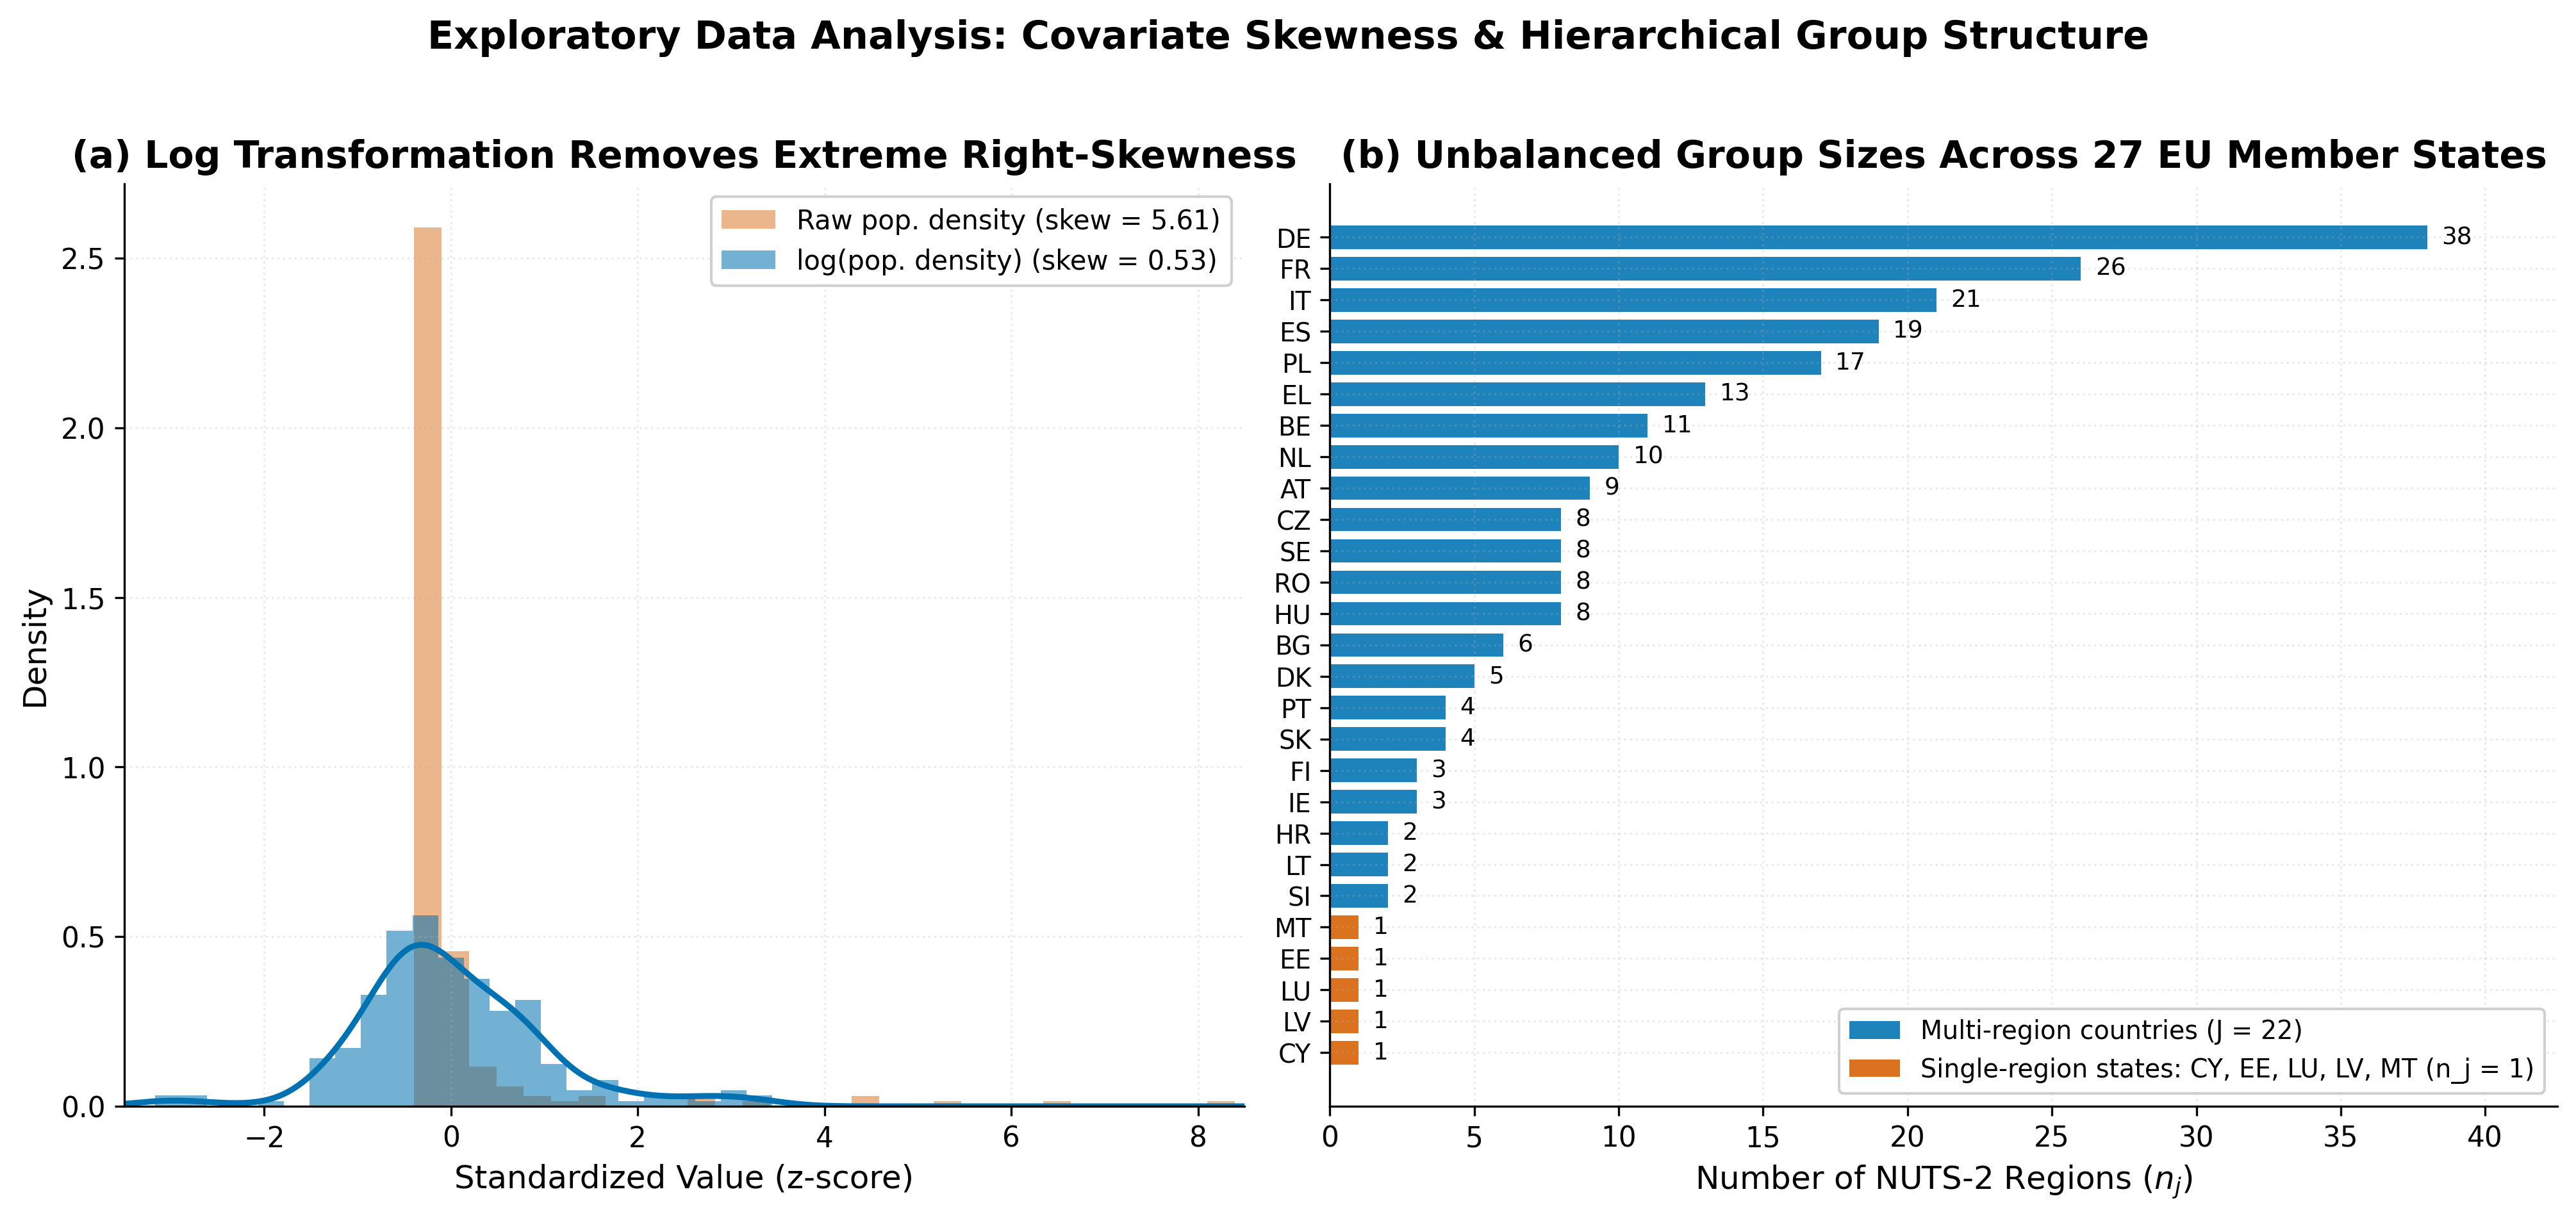
\includegraphics[width=0.82\textwidth]{02_eda_distributions_and_groups.png}
    \caption{Left: Natural-log transformation reduces population density skewness from $5.61$ to $0.53$. Right: Unbalanced NUTS-2 group sizes across 27 EU countries, highlighting the five single-region states (\texttt{CY}, \texttt{EE}, \texttt{LU}, \texttt{LV}, \texttt{MT}).}
    \label{fig:app_eda}
\end{figure}

\begin{figure}[H]
    \centering
    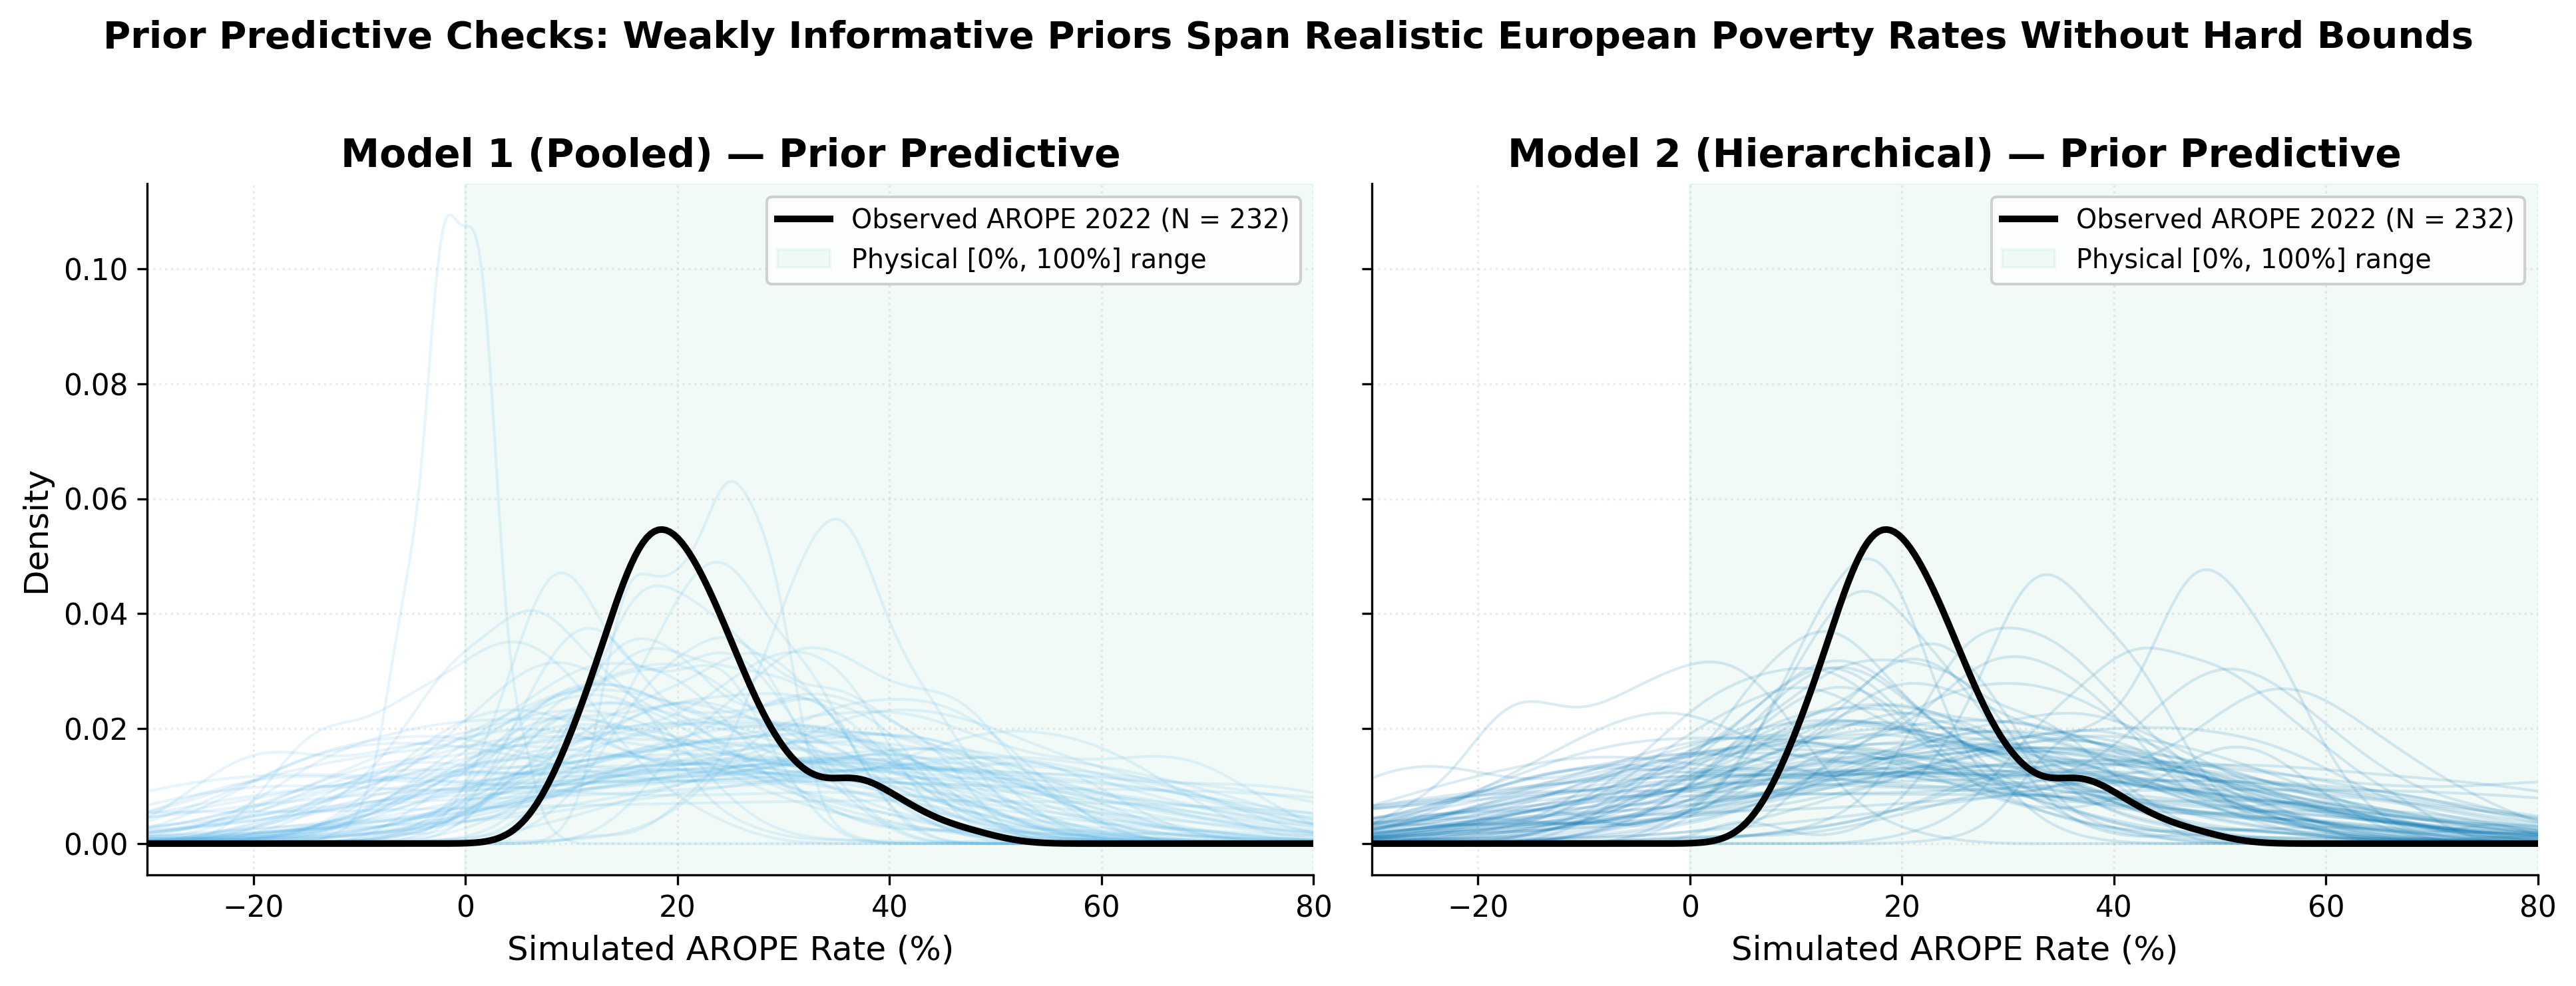
\includegraphics[width=0.82\textwidth]{03_prior_predictive_check.png}
    \caption{Prior predictive densities (80 draws each) on the original AROPE (\%) scale before conditioning on data. Both models place realistic prior mass across European poverty rates without hard artificial bounds.}
    \label{fig:app_prior}
\end{figure}

\begin{figure}[H]
    \centering
    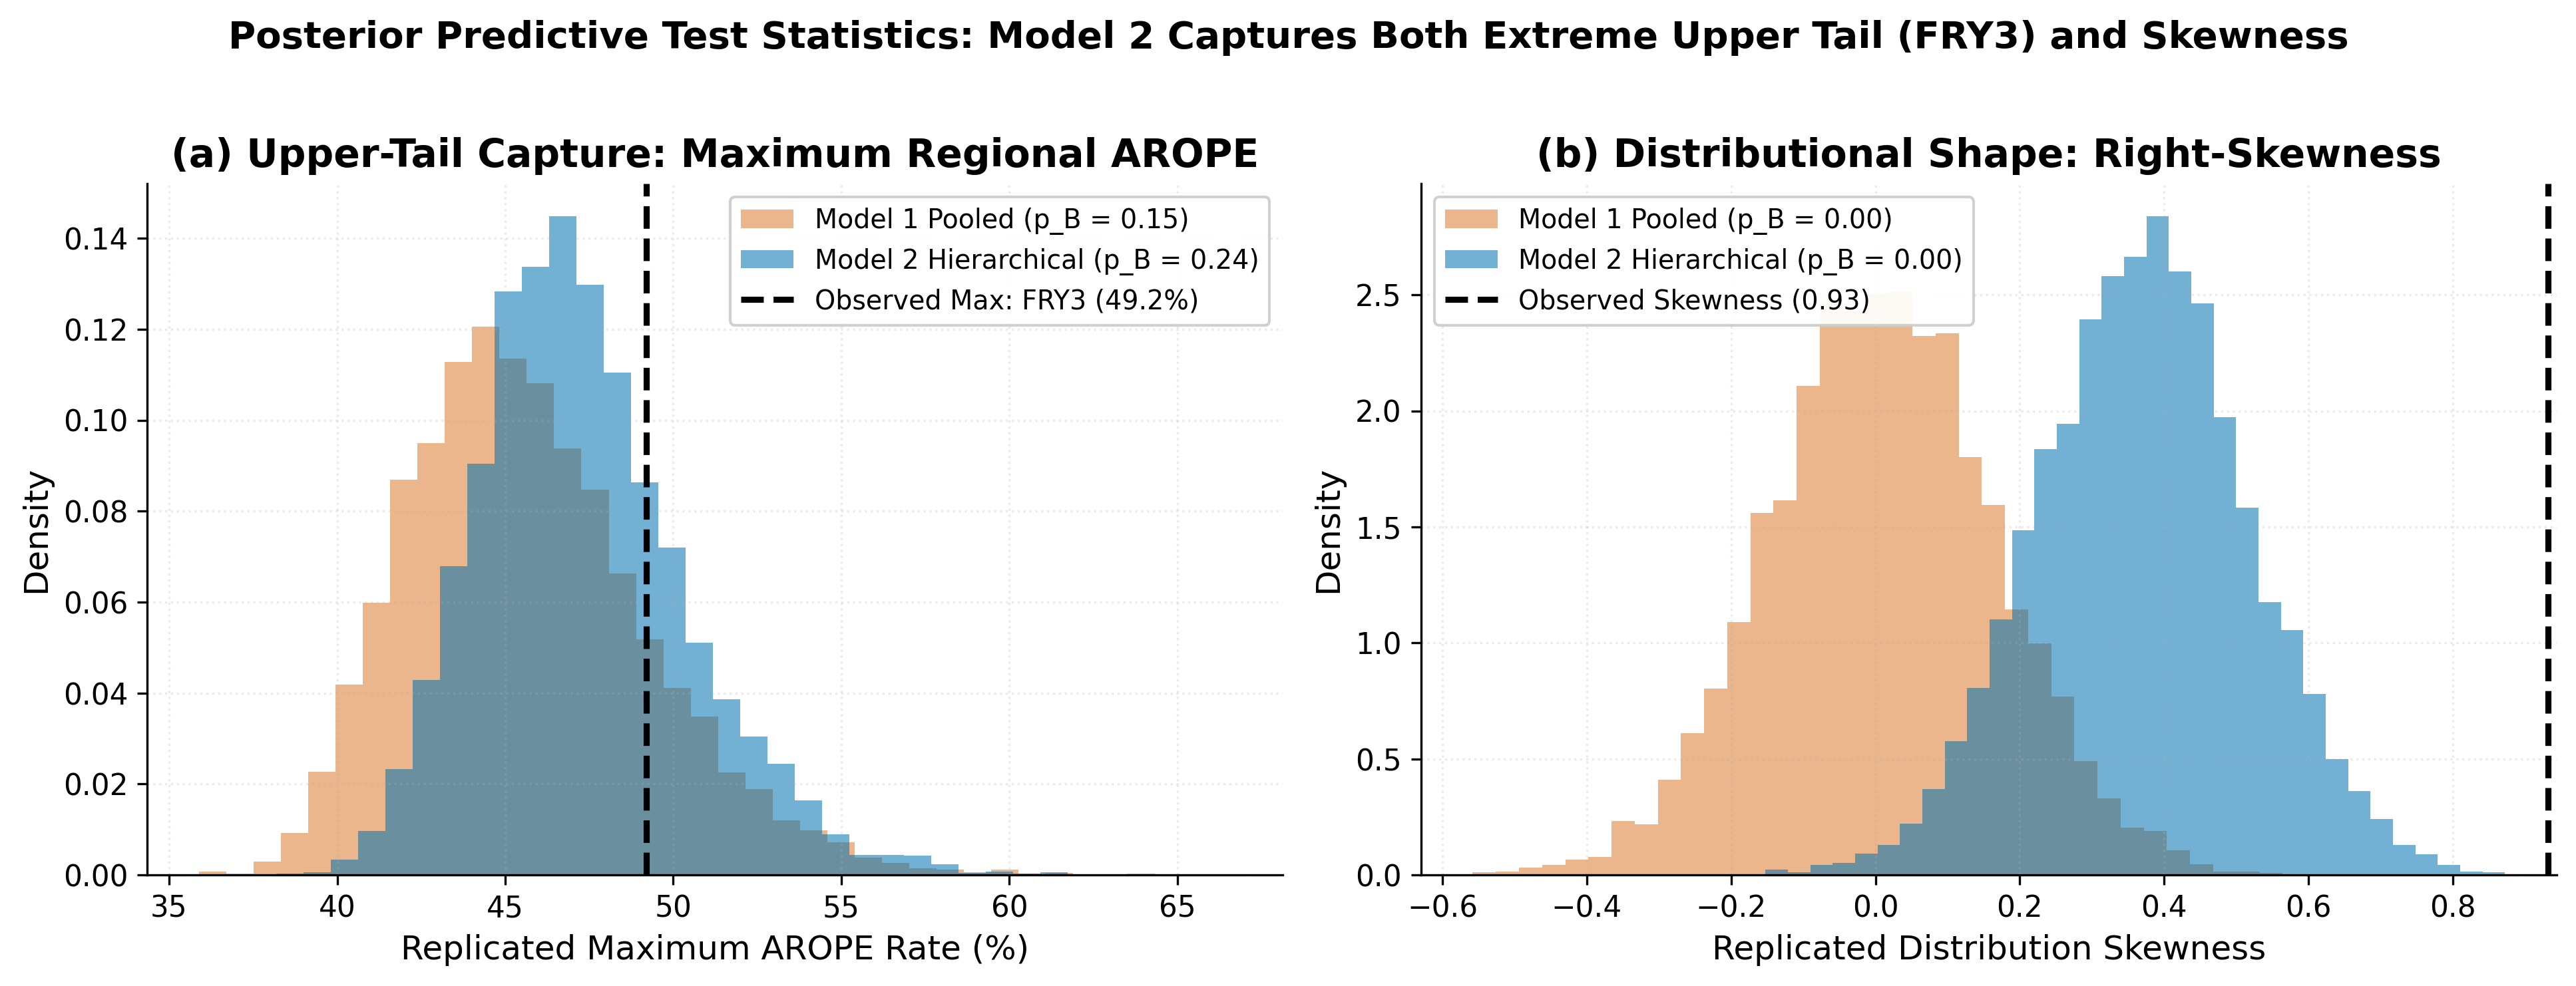
\includegraphics[width=0.82\textwidth]{06_ppc_test_statistics.png}
    \caption{Posterior predictive test statistics for maximum regional AROPE (left) and global skewness (right). Model~2 cleanly captures the upper-tail outlier \texttt{FRY3} ($49.2\%$, $p_B = 0.24$) and shifts skewness toward the observed $0.93$, though symmetric Gaussian residuals still underestimate full right-skewness.}
    \label{fig:app_ppc_stats}
\end{figure}

\begin{figure}[H]
    \centering
    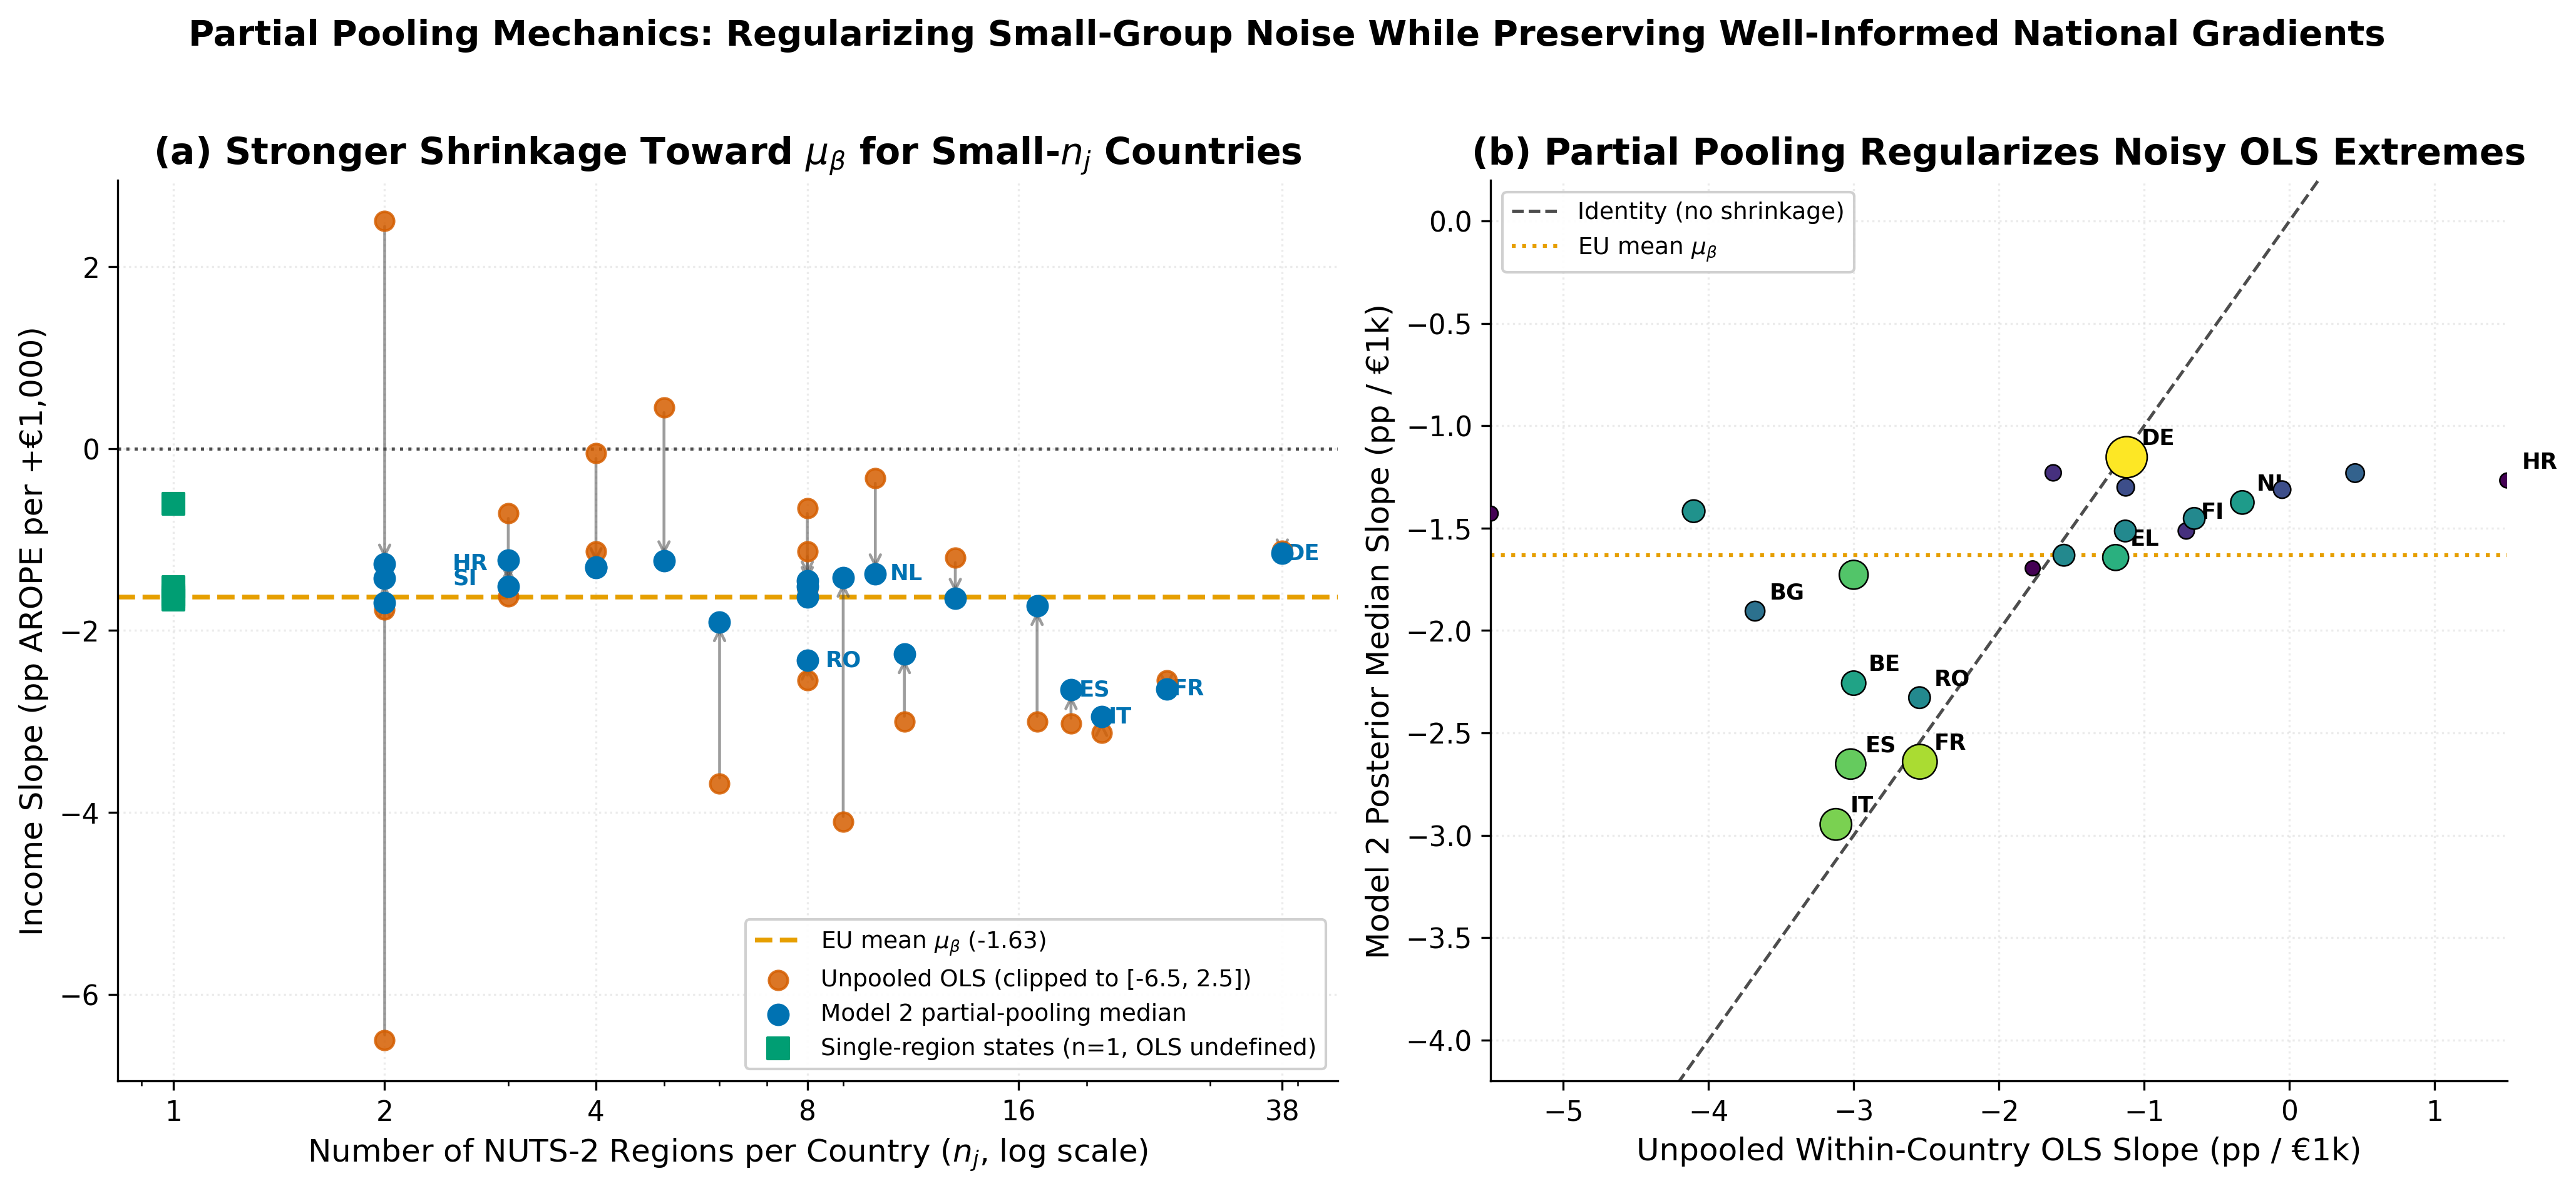
\includegraphics[width=0.82\textwidth]{11_partial_pooling_shrinkage.png}
    \caption{Partial-pooling shrinkage comparing unpooled within-country OLS against Model~2 posterior medians. Noisy small-$n_j$ OLS estimates are regularized toward $\mu_\beta = -1.63\text{ pp}$/\euro{}1k, well-informed countries retain their empirical gradients, and single-region states ($n_j = 1$) receive coherent estimates.}
    \label{fig:app_shrinkage}
\end{figure}

\end{document}
